\documentclass[11pt,a4j]{jreport}

\usepackage{comment}
\usepackage{float}
\usepackage{color}
\usepackage{multicol}
\usepackage{multirow}
\usepackage[dvipdfmx]{pict2e}
\usepackage{wrapfig}
\usepackage{graphicx}
\usepackage{bm}
\usepackage{url}
\usepackage{underscore}
\usepackage{colortbl}
\usepackage{tabularx}
\usepackage{fancyhdr}
\usepackage{ulem}
\usepackage{cite}
\usepackage{amsmath,amssymb,amsfonts}
\usepackage{algorithmic}
\usepackage{textcomp}
\usepackage{xcolor}
\usepackage[ipaex]{pxchfon}
\usepackage{pdfpages}
\usepackage{subcaption}
\usepackage{array}
\usepackage{adjustbox}
\usepackage{lipsum}

\usepackage[number-unit-product=~]{siunitx}

\usepackage[top=30truemm,bottom=30truemm,left=25truemm,right=25truemm]{geometry}

\renewcommand{\arraystretch}{1.2}

\begin{document}

\chapter{演奏実験}
反射音の到来方向が合唱者の演奏時の主観印象評価に与える影響について検討するため、第4章で生成した音場を用いて声楽カルテットによる演奏実験を行った。本章では、演奏実験の方法とその結果および考察について述べる。
%=======================================================================

\section{実験の概要}
図\ref{fig:実験音場のSTEarly}から図\ref{fig:実験音場の残響時間}に示すように、音場αからδの音響特性は近しく、その聴感的な印象の差異も残響時間が異なる場合のような極端な違いを感じさせるものとはなっておらず、各音場の印象の絶対評価では反射音到来方向の影響が適切に抽出できない可能性がある。そこで、本実験では、被験者に基準音場での演奏ののちに、基準音場から反射音の方向特性を変化させた音場αからδのうちいずれかの音場での演奏を行ってもらい、その印象の変化について回答を得る試行をαからδのすべての音場について繰り返すことで、反射音の到来方向特性を変化させたときの演奏時の印象の変化を調べることを試みた。

演奏実験はソプラノ、アルト、テノール、バスによる4人1組の混声四部の四重奏にて行った。被験者は合唱経験者31名(ソプラノ・アルト・バス8人、テノール7人。うち声楽経験者9名)であり、8組の実験グループを作成した。なお、実験グループのうち一つのグループでテノールに欠員が生じたため、そのグループにおいては筆者がテノールとして演奏に参加した。

実験には平易な日本語の混声四部合唱曲として「ふるさと」の一番を用いた。音場αからδの提示順序はランダムとした。並び順は一般的な混声四部のカルテットと同様に、舞台下手側として想定した方からソプラノ、アルト、テノール、バスの順とした。演奏実験の様子を図\ref{fig:演奏実験の様子}に示す。

\vspace{\stretch{1}}

\begin{figure}[H]
  \centering
  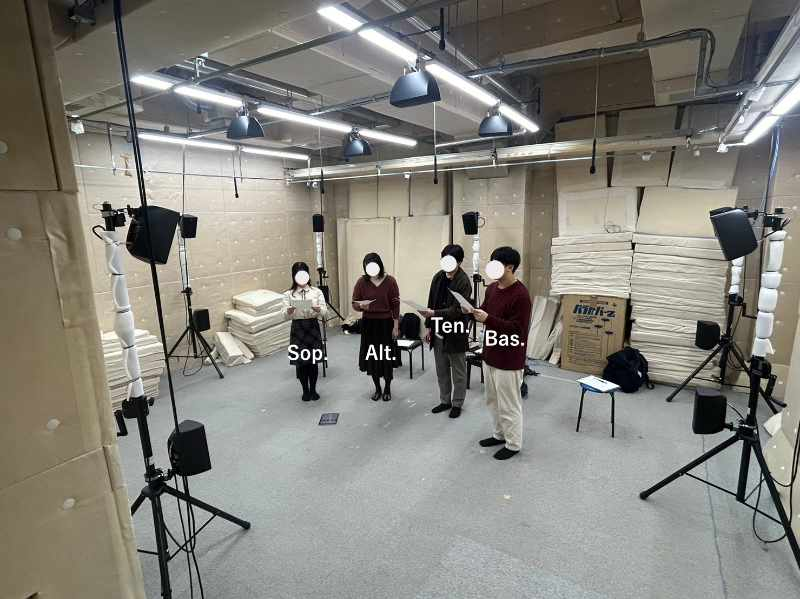
\includegraphics[width=0.6\linewidth]{images/subjectiveExp/chorusExpLowQ.jpg}
  \caption{演奏実験の様子}
  \label{fig:演奏実験の様子}
\end{figure}

\vspace{\stretch{1}}

%=======================================================================
\newpage

\section{方法}

\subsection{実験の手順}

実験の実施に先立ち、被験者に実験に関する説明を行い、実験の参加同意書およびフェイスシートの記入を求めた。その後、ウォーミングアップと曲の練習を行う時間を設け、「自身のパートを歌うことに一生懸命になりすぎず、他パートや空間の響きなどに意識が向けられる程度に習熟する」よう教示して各自のパートの音の確認およびアンサンブルの練習を求めた。練習の時間は厳密には区切らず、教示した習熟度に達した旨の申告を受け練習を終了した。練習の最後に、演奏実験の流れと評価項目について確認するため、基準音場での演奏ののちにランダムに一つ実験音場を提示して演奏する実験1条件あたりの流れを体験させた。

演奏実験では、基準音場と音場αからδの違いを評定尺度法による段階評価および自由記述による音場の印象の評価を行い、これを音場αからδすべてについて終えるまで繰り返した。実験全体の流れを表\ref{tab:実験全体の流れ}に、実験1条件あたりの流れを表\ref{tab:実験1条件あたりの流れ}に示す。

\subsection{音場の評価方法}
音場の評価は評定尺度法による段階評価と自由記述にて実施した。段階評価に用いた評価項目はGade\cite{Gade1989I}によりまとめられた演奏家のホールに対する6つの評価項目である、響き(Reverberance)、自分の音の聞きやすさ(Support)、音色(Timbre)、ダイナミクス(Dynamics)、互いの音の聞きやすさ(Hearing Each Other)、時差(Time Delay)を参考に決定した。

響き、自分の音の聞きやすさ、互いの音の聞きやすさに関する評価について、「響きが増えたか」「自分の音の聴きやすさ」「他人の音の聴きやすさ」を「響きの印象に関する項目」として設定した。

音色に関する評価として、本研究では「空間の印象」として具体化し、「空間の広がり」「客席全体に届く感じ」「自分に音が帰る感じ」「音に包まれる感じ」を設定した。また、時差についても空間の広がりを感じさせる要素として、本研究では空間印象に反映されるものとみなした。

ダイナミクスを含めた演奏の印象の評価について、「疲れ感」「強弱の付けやすさ」「アンサンブルのしやすさ」「音が溶け合う感じ」として設定した。

また、総合的な評価として、演奏の完成度自体に対する客観的な視点からの評価として「演奏がうまくいったか」、演奏の巧拙によらない自身の演奏時の感覚に基づく評価として「演奏のしやすさ」を設定した。

段階評価に用いた評価項目および評価尺度を表\ref{tab:段階評価の評価項目および評定尺度}に示す。また、評定尺度は-3から3までの7段階評価とした。さらに、すべての条件での演奏および評価が終了した後に、自由記述による全体を通した印象の評価を行った。

%=======================================================================
\newpage

\begin{table}[H]
  \centering
  \caption{実験全体の流れ}
  \label{tab:実験全体の流れ}

  \begingroup
  \renewcommand{\arraystretch}{1.2}

  \begin{tabular}{|c|c|}
    時間 & 内容 \\
    \hline
    0:00〜0:10 & 説明、同意書およびフェイスシートの記入 \\
    0:10〜0:25 & ウォーミングアップ・音取り・アンサンブル練習・評価練習 \\
    0:25〜0:30 & 1回目の演奏実験(基準音場→αからδのうち一つの音場)と評価 \\
    0:30〜0:35 & 2回目の演奏実験(基準音場→αからδのうち一つの音場)と評価 \\
    0:35〜0:40 & 3回目の演奏実験(基準音場→αからδのうち一つの音場)と評価 \\
    0:40〜0:45 & 4回目の演奏実験(基準音場→αからδのうち一つの音場)と評価 \\
    0:45〜0:50 & 全体を通した評価\\
    0:50〜0:55 & 回答用紙を回収して終了 \\
  \end{tabular}
  \endgroup
\end{table}

\vspace{1\baselineskip}

\begin{table}[H]
  \centering
  \caption{実験1条件あたりの流れ}
  \label{tab:実験1条件あたりの流れ}

  \begingroup
  \renewcommand{\arraystretch}{1.2}

  \begin{tabular}{|m{3cm}|m{3cm}|m{9cm}|}
    \multicolumn{1}{|c|}{基準音場で演奏} &
    \begin{tabular}{c}音場α〜δの\\いずれかで演奏
    \end{tabular}
    & \multicolumn{1}{c|}{響きの印象の変化を評価} \\
    \hline
    \multicolumn{1}{|c|}{1分} & \multicolumn{1}{c|}{1分} & \multicolumn{1}{c|}{3分} \\ 
  \end{tabular}
  \endgroup
\end{table}

\vspace{1\baselineskip}

\begin{table}[H]
  \centering
  \caption{段階評価の評価項目および評定尺度}
  \label{tab:段階評価の評価項目および評定尺度}

  \begingroup
  \renewcommand{\arraystretch}{1.2}
  \begin{tabular}{c|c|c}
    & 評価項目 & 評定尺度($-3$ 〜 $3$の7段階) \\
    \hline \hline

    \multirow{3}{*}{音場の印象} & 響きが増えたか & 減った / 増えた \\
    \cline{2-3}
    & 自分の音の聴きやすさ & \multirow{2}{*}{聴きやすくなった / 聴きにくくなった}\\
    \cline{2-2}
    & 他人の音の聴きやすさ & \\
    \hline \hline

    \multirow{4}{*}{空間の印象} & 空間の広がり & 狭くなった / 広くなった \\
    \cline{2-3}
    & 客席全体に届く感じ & \multirow{3}{*}{減った / 増えた} \\
    \cline{2-2}
    & 自分に音が返る感じ & \\
    \cline{2-2}
    & 音に包まれる感じ & \\
    \hline \hline

    \multirow{4}{*}{演奏の印象} & 疲れ感 & 疲れやすくなった / 疲れにくくなった \\
    \cline{2-3}
    & 強弱のつけやすさ & つけやすくなった / つけにくくなった \\
    \cline{2-3}
    & アンサンブルのしやすさ & しにくくなった / しやすくなった\\
    \cline{2-3}
    & 音が溶け合う感じ & 減った / 増えた \\
    \hline \hline

    \multirow{2}{*}{総合的な印象} & 演奏がうまくいったか & うまくいかなかった / うまくいった \\
    \cline{2-3}
    & 演奏のしやすさ & しにくくなった / しやすくなった \\
    \hline

  \end{tabular}
  \endgroup
\end{table}

%=======================================================================
\clearpage
\section{結果と考察}

評定尺度法による段階評価における全被験者(N = 31)の評点平均と標準偏差(エラーバー)を図\ref{fig:評定尺度法による段階評価の平均値と標準偏差}に示す。また段階評価の各項目について「平均値が0に等しい」ことを帰無仮説とするt検定(両側検定)を行なったところ、いくつかの項目で有意差が検出されたため、0.01 ≦ p < 0.05 の項目を*、p < 0.01 の項目を**として検定結果を図中に併せて示す。

\subsection{全体的な傾向}

全体的に評価の平均値は0以上の値になっているが、\ref{fig:実験音場のSTEarly}から\ref{fig:実験音場の残響時間}に示すように音場αからδの響きはわずかに基準音場よりも増加していることため、このことが影響している可能性がある。しかし$\mathrm{ST_{Early}}$および$\mathrm{ST_{Late}}$は実験音場間での差異が小さく、また残響時間の伸長の程度は音場βで最も大きいにもかかわらず、音場βの評価の平均値は他の音場と比較して低い値となっている。このことから、残響時間の伸長や$\mathrm{ST_{Early}}$、$\mathrm{ST_{Late}}$の違いではなく、反射音到来方向の変化が響きの増加感に影響を与えている可能性が示唆される。

全体の傾向として、平均値は1以下と小さい値となった。特に、初期反射音の方向特性に変化を与えた音場αと音場βではほとんどすべての評価項目で0.5以下の値となった。初期反射音は$\SI{0.1}{\second}$以内というごく短い時間に到来するため、主観印象への影響は音色の変化として生じることが多く、大きな音色の変化を伴わない方向特性の変化が知覚されにくかったためと考えられる。

\subsubsection*{各評価項目の結果と考察}

響きの印象についての三項目のうち、「響きが増えたか」では音場α、音場γ、音場δで基準音場よりも評価が高くなる傾向が見られた。音場βは後方からの初期反射音を増強した音場で、後壁からの初期反射音供給が多い現実の音場を模している基準音場と似通った方向特性となっているが、音場α、γ、δは方向特性の変化が音場βよりも大きく、音場βの方向特性の変化の小ささが残響時間の伸長の割に響きの増加感に影響を与えなかったのではないかと考えられる。

また、「自分が発した音の聴きやすさ」についてはいずれの実験音場でも基準音場に対する有意差は検出されなかったが、「他人が発した音の聴きやすさ」については前方からの後期反射音を増強させた音場γで評価が高くなった。このことから、前方からの後期反射音の増強が他人の音の聴きやすさに対して有意な影響を与えることが示唆される。

空間の印象について、「空間の広がり」「客席全体に届いている感じ」で音場γの評価が高くなった。音場γは前方からの後期反射音を増強させた音場で、前方からの後期反射音の増強が空間の広がりや客席全体に届いている感じに対して有意な影響を与えることが示唆される。
  
演奏の印象について、「疲れ感」の評価については、平均値はほぼ0であり、また標準偏差もたの評価項目に比べて比較的小さい値となっており、方向特性による影響はほとんどないと考えられる。響きの印象および空間の印象においても評価の高い傾向が見られた音場γでは、「強弱のつけやすさ」「アンサンブルのしやすさ」においても評価が高く、前方からの後期反射音が演奏者にとって好ましい変化をもたらすことが示唆される。また、「アンサンブルのしやすさ」では後方からの後期反射音を増強した音場δでも有意差が検出された。

総合的な評価については有意差は検出されず、上述した評価が演奏の巧拙や主観的な好みによらないことが示唆された。
  
%=======================================================================
\newpage
\begin{figure}[H]
  \centering
  
  \begin{minipage}{1\linewidth}
    \centering
    
\includegraphics[scale=.55]{images/subjectiveExp/statisticAnalysis/legend.pdf}
    \label{fig:段階評価の凡例}
  \end{minipage}

  \vspace{1\baselineskip}

  \begin{minipage}{1\linewidth}
    \centering
    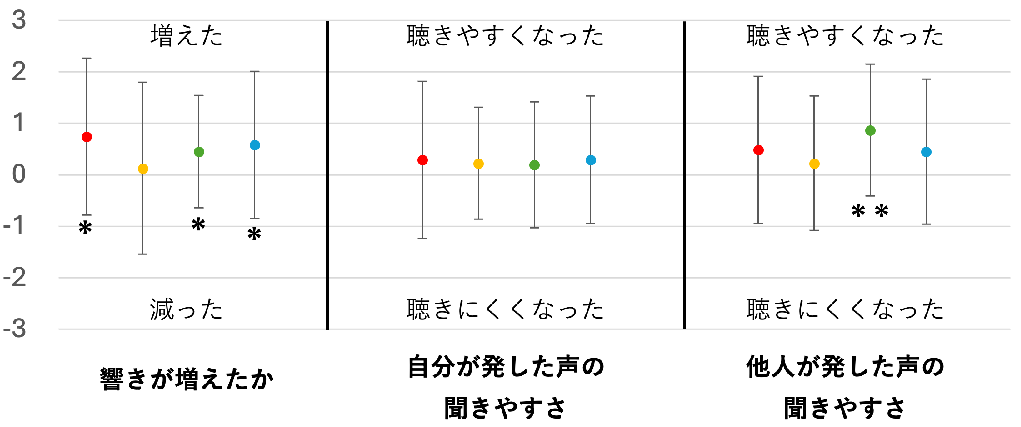
\includegraphics[scale=.55]{images/subjectiveExp/statisticAnalysis/01reverb_a.pdf}
    \caption*{響きの印象}
    \label{fig:響きの印象}
  \end{minipage}
  \\
  \vspace{1\baselineskip}
  \begin{minipage}{1\linewidth}
    \centering
    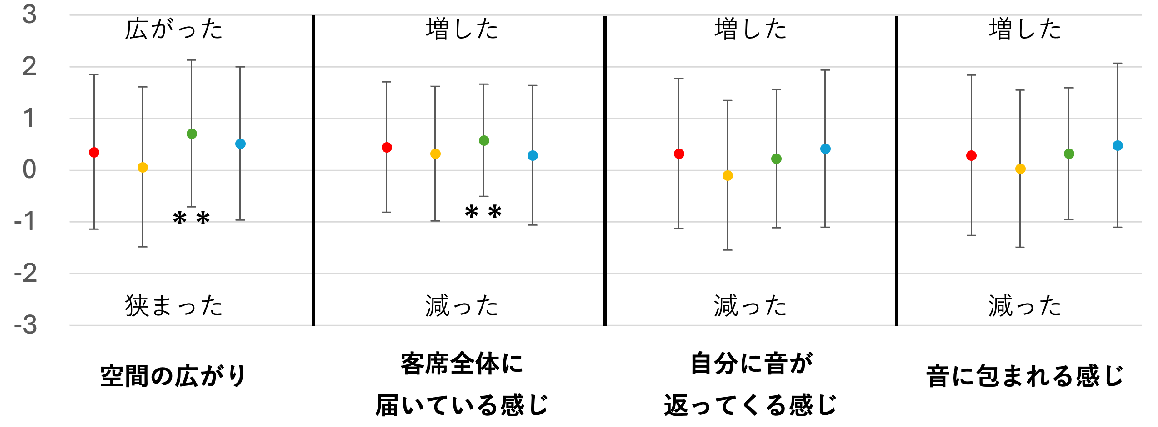
\includegraphics[scale=.55]{images/subjectiveExp/statisticAnalysis/02space_a.pdf}
    \caption*{空間の印象}
    \label{fig:空間の印象}
  \end{minipage}
  \\
  \vspace{1\baselineskip}
  \begin{minipage}{1\linewidth}
    \centering
    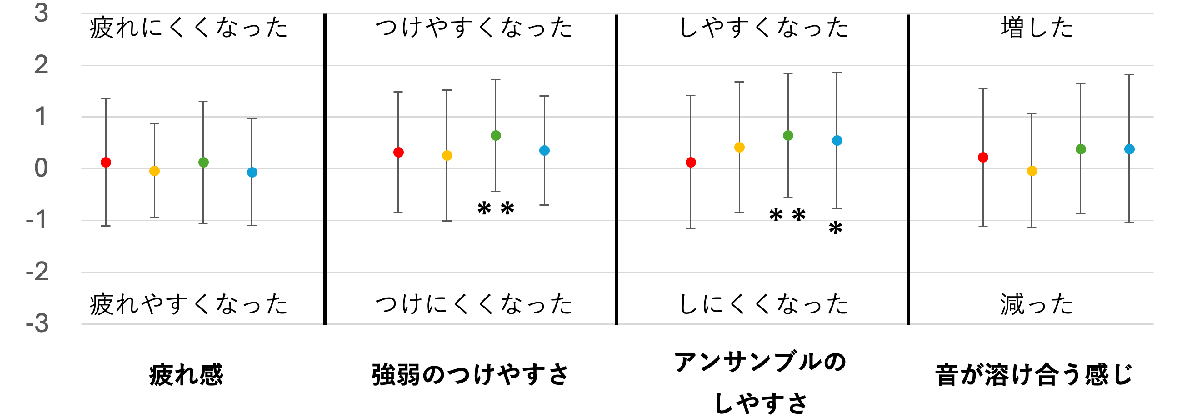
\includegraphics[scale=.55]{images/subjectiveExp/statisticAnalysis/03performance_a.pdf}
    \caption*{演奏の印象}
    \label{fig:演奏の印象}
  \end{minipage}
\\
  \vspace{1\baselineskip}
  \begin{minipage}{1\linewidth}
    \centering
    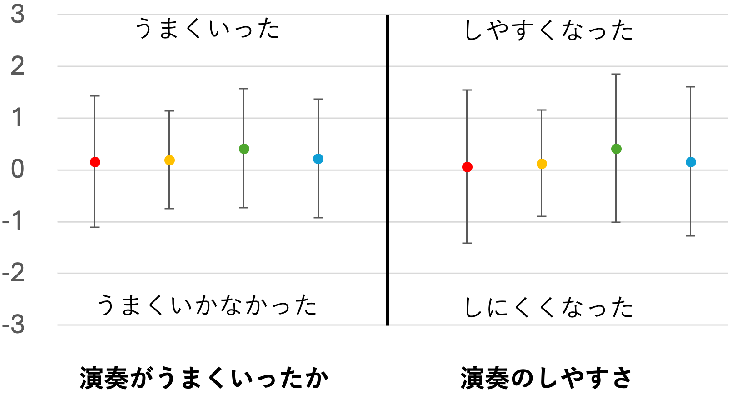
\includegraphics[scale=.55]{images/subjectiveExp/statisticAnalysis/04overall_a.pdf}
    \caption*{総合的な評価}
    \label{fig:総合的な評価}
  \end{minipage}

  \caption{評定尺度法による段階評価の平均値と標準偏差(* p < 0.05 \hspace{5mm} ** p < 0.01)}
  \label{fig:評定尺度法による段階評価の平均値と標準偏差}
\end{figure}

%=======================================================================
\newpage

\subsection{パートによる評価の違い}
本実験では、演奏時の条件を現実的な条件に近いものとするため、標準的な混声四部のカルテットの並び順に倣い、舞台下手側と想定したからソプラノ・アルト・テノール・バスの順の並びとした。演奏者のパートにより、自身の音域や立ち位置、アンサンブルにおける音楽上の役割が
異なっているため、パートによって評価に異なった傾向が現れる可能性がある。そこで、パートによる評価の違いを調べるため、パートごとの評点平均と標準偏差を計算した。この結果を図\ref{fig:パートごとの響きの印象に関する評価}から図\ref{fig:パートごとの総合的な評価}に各音場ごとに示す。

段階評価の各項目について「平均値が0に等しい」ことを帰無仮説とするt検定(両側検定)を行なったところ、いくつかの項目で有意差が検出された。また、同一の音場での同一の評定項目に対するすべてのパートの組み合わせについて、「評定平均が等しい」ことを帰無仮説とするステューデントのt検定を行なったところ、いくつかの項目で有意差が検出された。これらの検定結果について、0.01 ≦ p < 0.05 の項目を*、p < 0.01 の項目を**として図中に併せて示す。

\subsubsection*{初期反射音に関する評価}
全体での評価において、初期反射音の方向特性に変化を与えた音場αと音場βではほとんどすべての評価項目で0.5以下の値となっていた。パートごとの評価をみた場合であっても、音場βへの評価で有意差が検出された項目は「他人が発した音の聴きやすさ」に対するバスパートの評価のみであり、後方からの初期反射音の供給量の変化はどのパートに対しても顕著な聴感印象の変化を与えないことが示唆される。一方で、音場αに対する評価では、「アンサンブルのしやすさ」「響きが溶け合う感じ」「演奏がうまくいったか」「演奏のしやすさ」の評価項目にてパート間の有意差が検出され、これらのいずれの評価項目でもソプラノ・テノールからの評価が高く、アルト・バスからの評価が低くなる傾向が見られ、前方からの初期反射音の供給量の変化がパート間の感じ方の差異を生じさせたことが示唆された。

\subsubsection*{後期反射音に関する評価}
全体での評価において、「他人が発した音の聴きやすさ」「空間の広がり」「客席全体に届いている感じ」「強弱のつけやすさ」「アンサンブルのしやすさ」で高い評価を得た音場γは、これ以外の評価項目も含め、多くの評価項目において、ソプラノ・バスからの評価が高く、アルト・テノールからの評価が低くなる傾向が見られた。逆に、音場δでは、多くの評価項目においてソプラノ・バスからの評価は低く、テノール・アルトからの評価が高くなる傾向が見られた。これにより、後期反射音の方向特性は、その偏りが前後のどちらであっても各演奏者に対して何らかの差異を感じさせている可能性が高いことが示唆された。

パートごとの評価の傾向の違いを生じさせる原因についてさらに考察するため、次節にて個々人の評価を散布図としてプロットして検討する。

%=======================================================================
\newpage
\begin{figure}[H]
  \centering
  
  \begin{minipage}{1\linewidth}
    \centering
    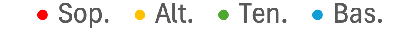
\includegraphics[scale=.55]{images/subjectiveExp/statisticAnalysis/part_legend.pdf}
  \end{minipage}
  \vspace{.5\baselineskip}

  \begin{minipage}{1\linewidth}
    \centering
    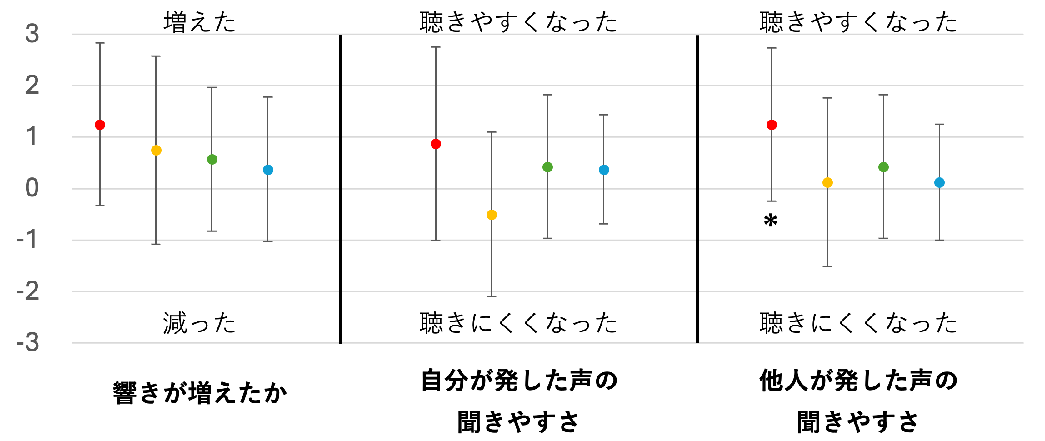
\includegraphics[scale=.55]{images/subjectiveExp/statisticAnalysis/part_reverb_a.pdf}
    \caption*{音場α}
    \label{fig:響きの印象α}
  \end{minipage}
  \\
  \vspace{1\baselineskip}
  \begin{minipage}{1\linewidth}
    \centering
    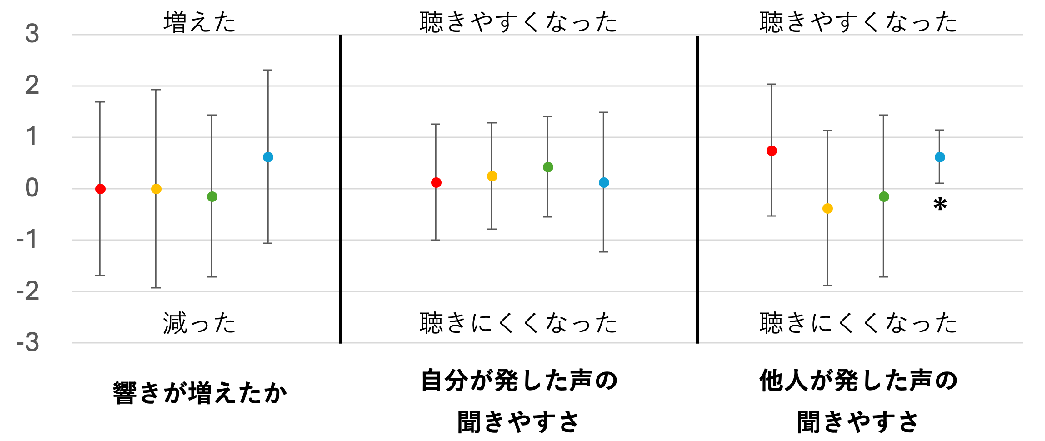
\includegraphics[scale=.55]{images/subjectiveExp/statisticAnalysis/part_reverb_b.pdf}
    \caption*{音場β}
    \label{fig:響きの印象β}
  \end{minipage}
  \\
  \vspace{1\baselineskip}
  \begin{minipage}{1\linewidth}
    \centering
    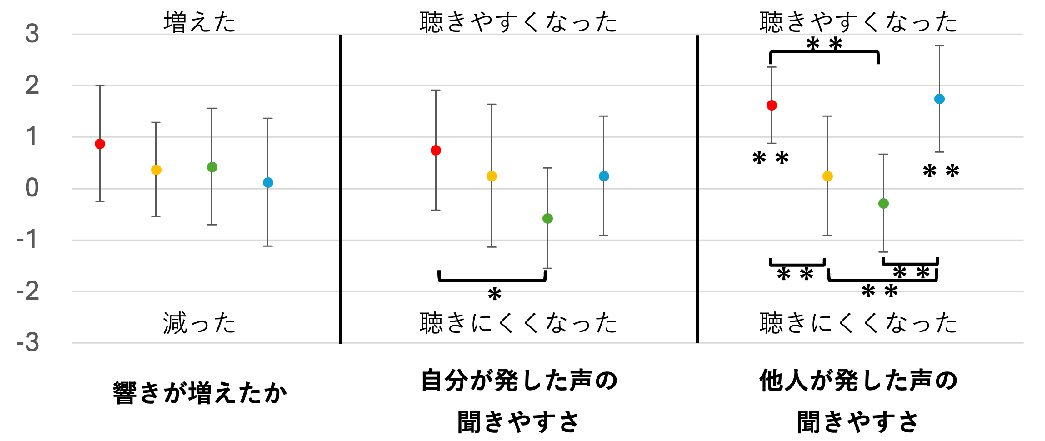
\includegraphics[scale=.55]{images/subjectiveExp/statisticAnalysis/part_reverb_c.pdf}
    \caption*{音場γ}
    \label{fig:響きの印象γ}
  \end{minipage}
  \\
  \vspace{1\baselineskip}
  \begin{minipage}{1\linewidth}
    \centering
    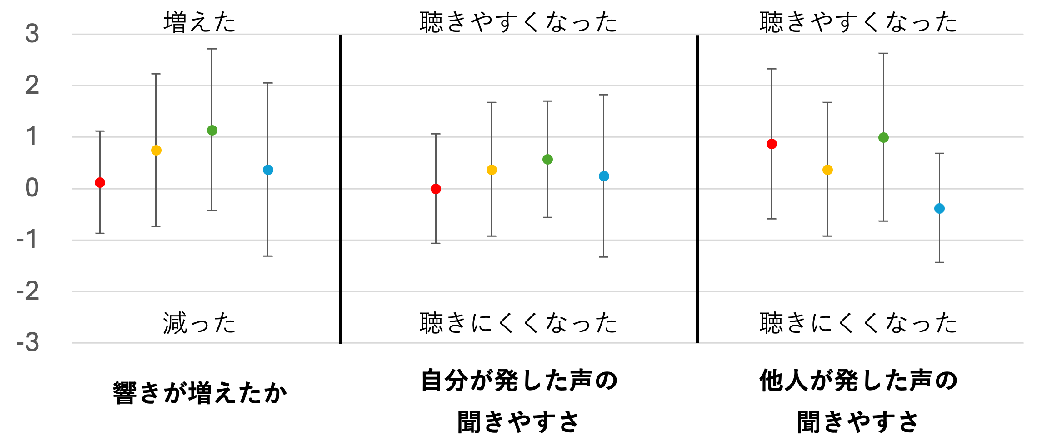
\includegraphics[scale=.55]{images/subjectiveExp/statisticAnalysis/part_reverb_d.pdf}
    \caption*{音場δ}
    \label{fig:響きの印象δ}
  \end{minipage}
  
  \caption{パートごとの響きの印象に関する評価}
  \label{fig:パートごとの響きの印象に関する評価}
\end{figure}

%=======================================================================

\newpage

\begin{figure}[H]
  \centering
  
  \begin{minipage}{1\linewidth}
    \centering
    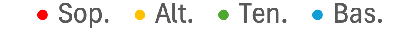
\includegraphics[scale=.55]{images/subjectiveExp/statisticAnalysis/part_legend.pdf}
  \end{minipage}
  \vspace{.5\baselineskip}

  \begin{minipage}{1\linewidth}
    \centering
    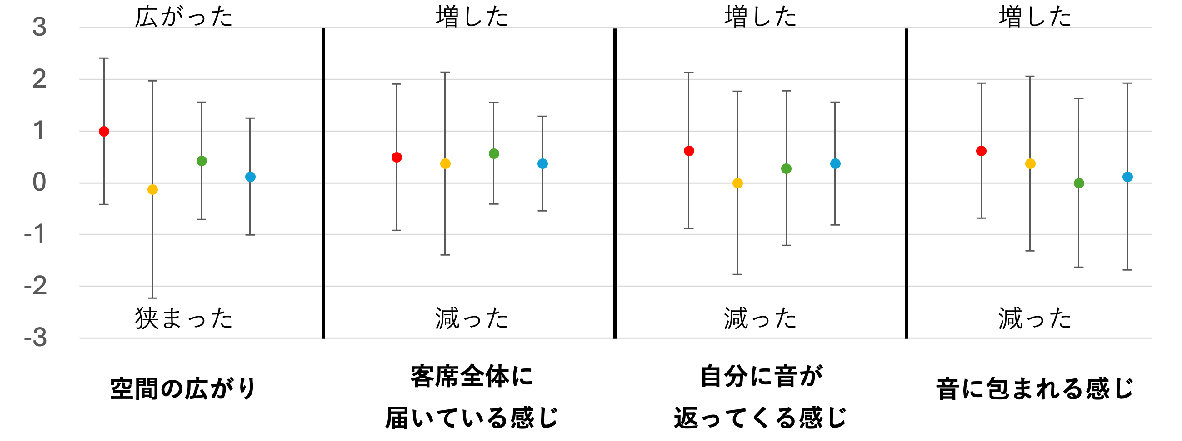
\includegraphics[scale=.55]{images/subjectiveExp/statisticAnalysis/part_space_a.pdf}
    \caption*{音場α}
    \label{fig:空間の印象α}
  \end{minipage}
  \\
  \vspace{1\baselineskip}
  \begin{minipage}{1\linewidth}
    \centering
    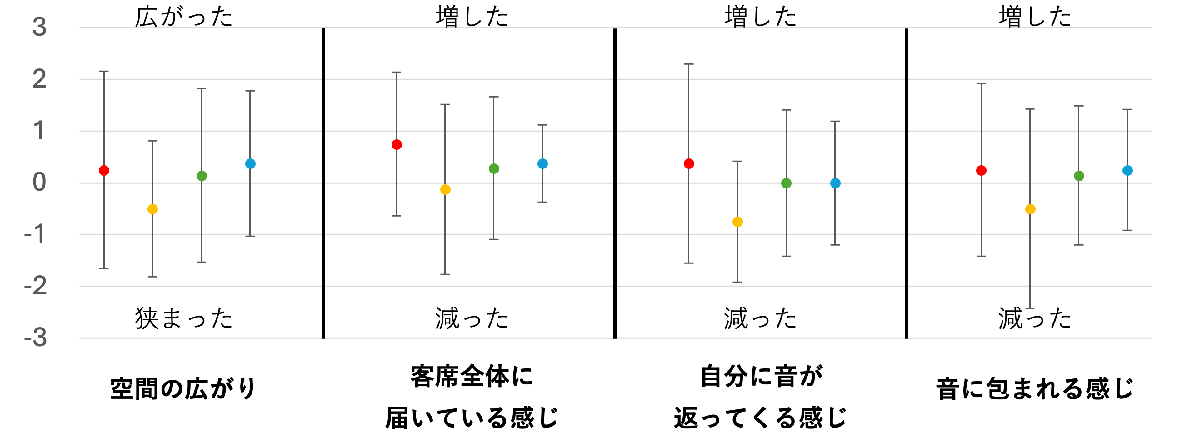
\includegraphics[scale=.55]{images/subjectiveExp/statisticAnalysis/part_space_b.pdf}
    \caption*{音場β}
    \label{fig:空間の印象β}
  \end{minipage}
  \\
  \vspace{1\baselineskip}
  \begin{minipage}{1\linewidth}
    \centering
    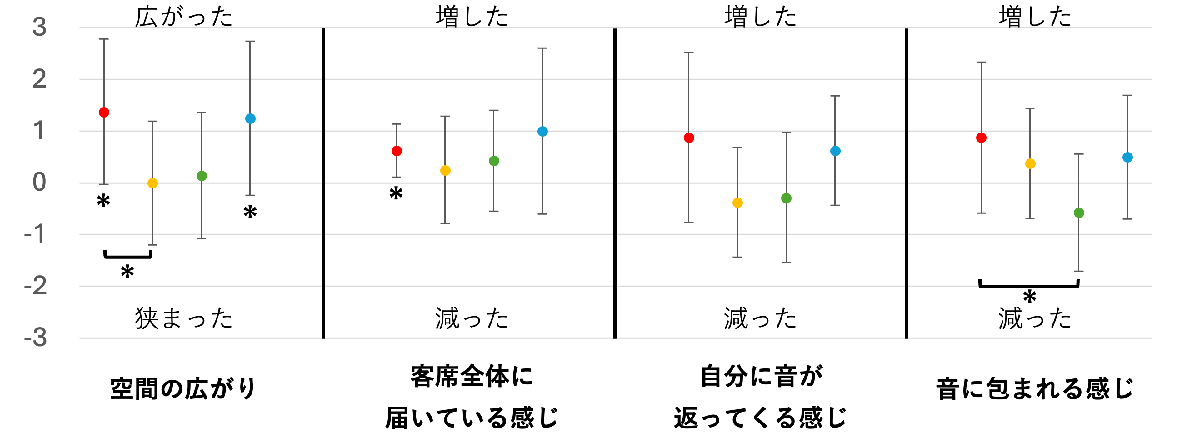
\includegraphics[scale=.55]{images/subjectiveExp/statisticAnalysis/part_space_c.pdf}
    \caption*{音場γ}
    \label{fig:空間の印象γ}
  \end{minipage}
  \\
  \vspace{1\baselineskip}
  \begin{minipage}{1\linewidth}
    \centering
    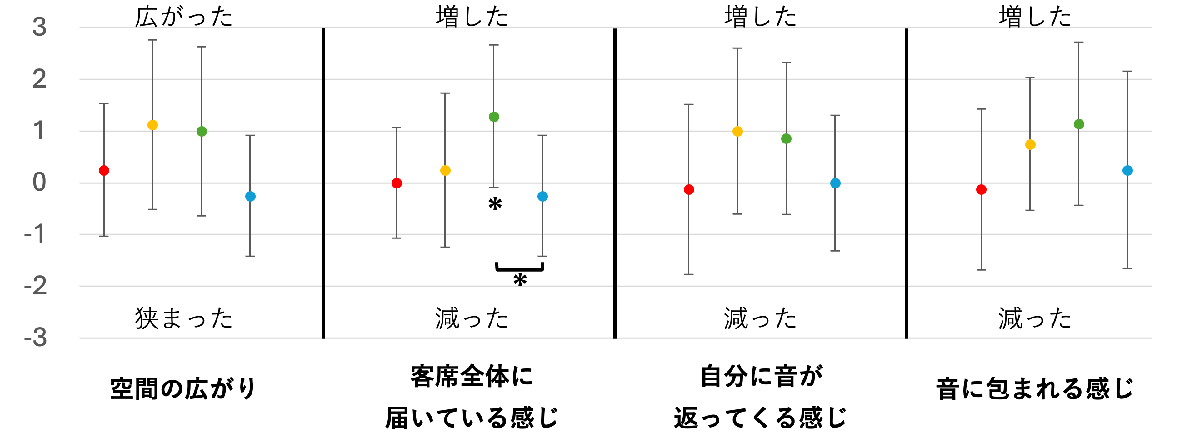
\includegraphics[scale=.55]{images/subjectiveExp/statisticAnalysis/part_space_d.pdf}
    \caption*{音場δ}
    \label{fig:空間の印象δ}
  \end{minipage}
  
  \caption{パートごとの空間の印象に関する評価}
  \label{fig:パートごとの空間の印象に関する評価}
\end{figure}
%=======================================================================

\newpage
\begin{figure}[H]
  \centering
  
  \begin{minipage}{1\linewidth}
    \centering
    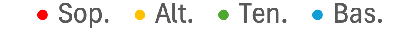
\includegraphics[scale=.55]{images/subjectiveExp/statisticAnalysis/part_legend.pdf}
  \end{minipage}
  \vspace{.5\baselineskip}

  \begin{minipage}{1\linewidth}
    \centering
    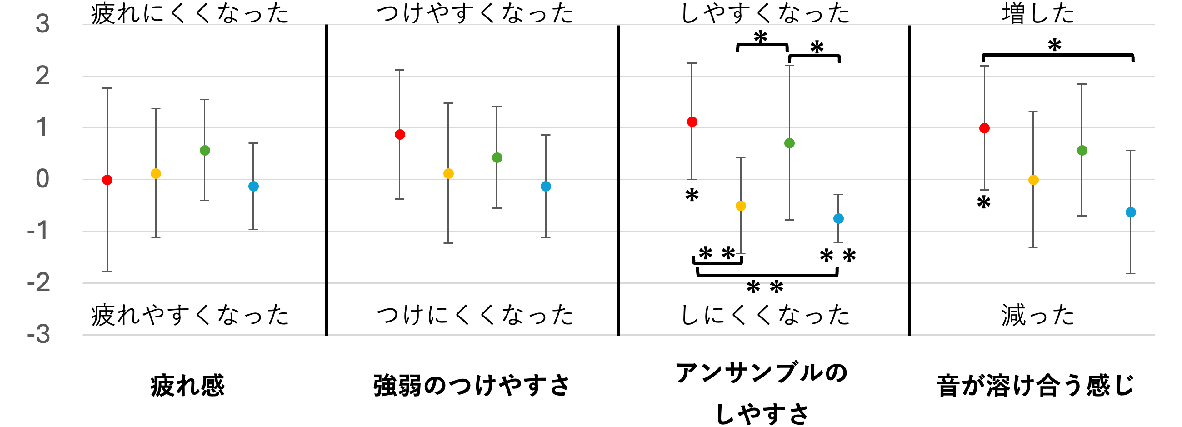
\includegraphics[scale=.55]{images/subjectiveExp/statisticAnalysis/part_performance_a.pdf}
    \caption*{音場α}
    \label{fig:演奏の印象α}
  \end{minipage}
  \\
  \vspace{1\baselineskip}
  \begin{minipage}{1\linewidth}
    \centering
    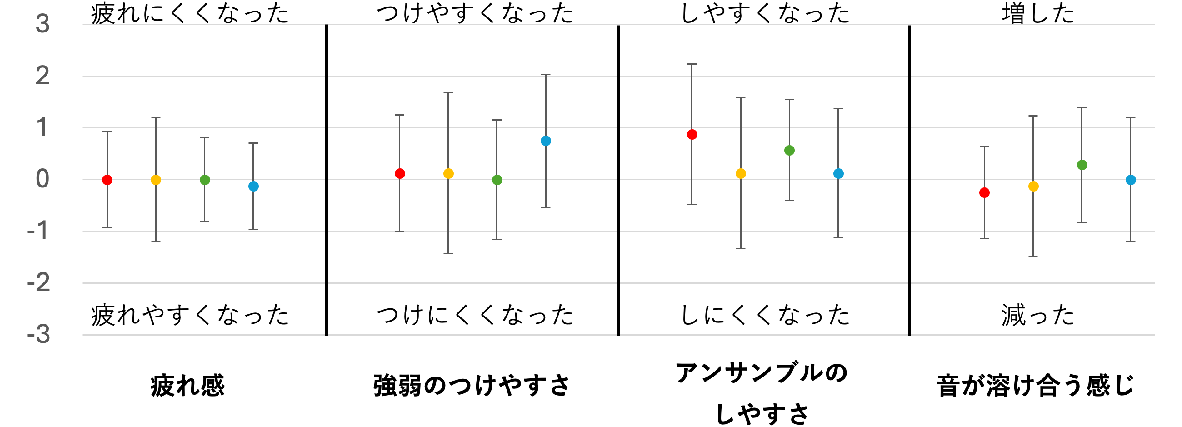
\includegraphics[scale=.55]{images/subjectiveExp/statisticAnalysis/part_performance_b.pdf}
    \caption*{音場β}
    \label{fig:演奏の印象β}
  \end{minipage}
  \\
  \vspace{1\baselineskip}
  \begin{minipage}{1\linewidth}
    \centering
    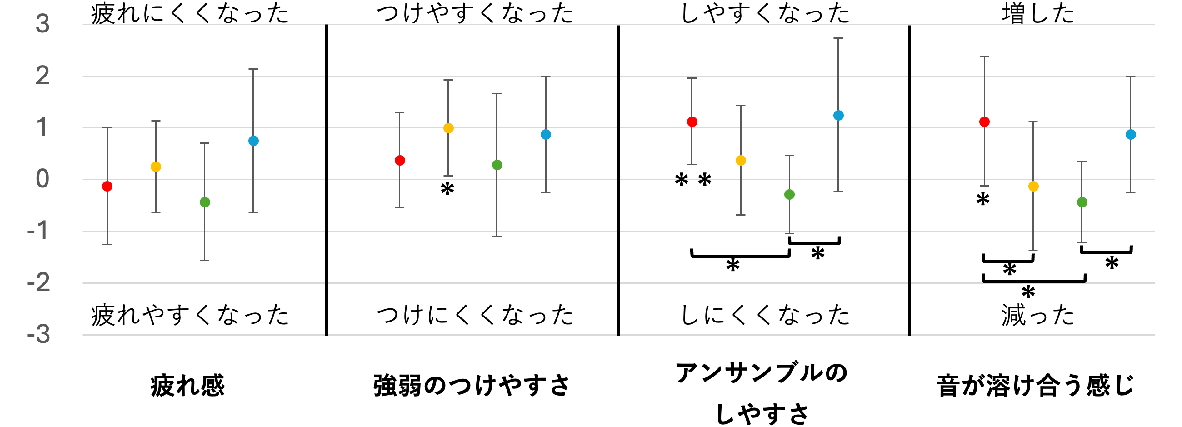
\includegraphics[scale=.55]{images/subjectiveExp/statisticAnalysis/part_performance_c.pdf}
    \caption*{音場γ}
    \label{fig:演奏の印象γ}
  \end{minipage}
  \\
  \vspace{1\baselineskip}
  \begin{minipage}{1\linewidth}
    \centering
    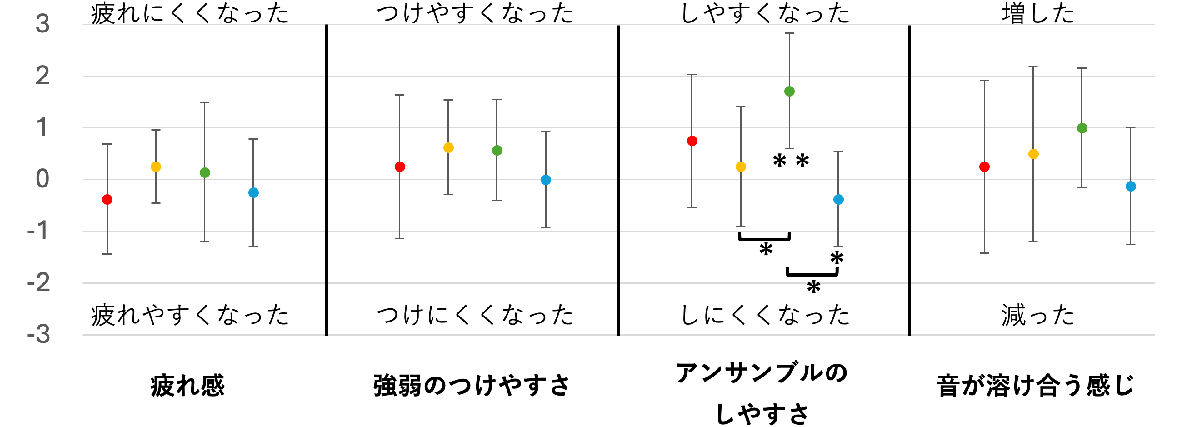
\includegraphics[scale=.55]{images/subjectiveExp/statisticAnalysis/part_performance_d.pdf}
    \caption*{音場δ}
    \label{fig:演奏の印象δ}
  \end{minipage}
  
  \caption{パートごとの演奏の印象に関する評価}
  \label{fig:パートごとの演奏の印象に関する評価}
\end{figure}

%=======================================================================
\newpage

\vspace*{\stretch{1}}
\begin{figure}[H]
  \centering
  
  \begin{minipage}{1\linewidth}
    \centering
    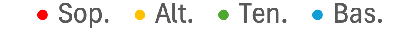
\includegraphics[scale=.55]{images/subjectiveExp/statisticAnalysis/part_legend.pdf}
  \end{minipage}

  \vspace{.5\baselineskip}

  \begin{minipage}{.5\linewidth}
    \centering
    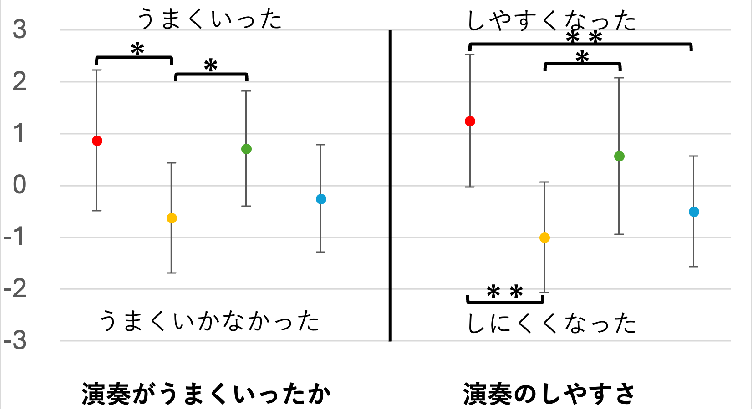
\includegraphics[scale=.55]{images/subjectiveExp/statisticAnalysis/part_overall_a.pdf}
    \caption*{音場α}
    \label{fig:総合的な評価α}
  \end{minipage}%
  \begin{minipage}{.5\linewidth}
    \centering
    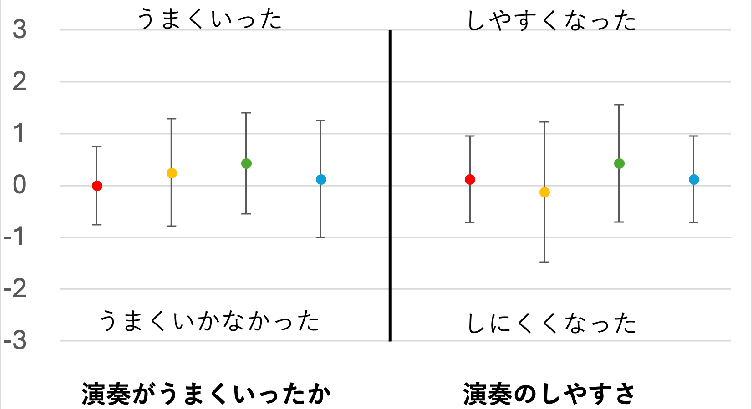
\includegraphics[scale=.55]{images/subjectiveExp/statisticAnalysis/part_overall_b.pdf}
    \caption*{音場β}
    \label{fig:総合的な評価β}
  \end{minipage}

  \vspace{1\baselineskip}

  \begin{minipage}{.5\linewidth}
    \centering
    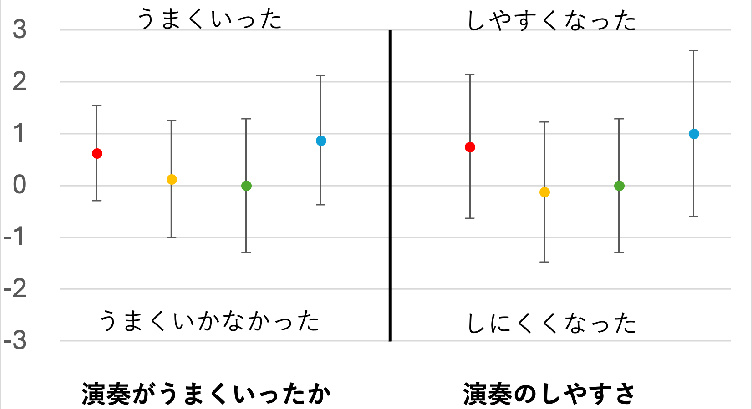
\includegraphics[scale=.55]{images/subjectiveExp/statisticAnalysis/part_overall_c.pdf}
    \caption*{音場γ}
    \label{fig:総合的な評価γ}
  \end{minipage}%
  \begin{minipage}{.5\linewidth}
    \centering
    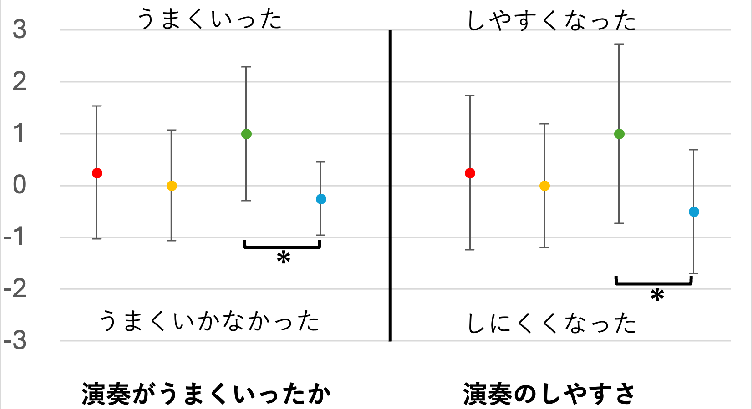
\includegraphics[scale=.55]{images/subjectiveExp/statisticAnalysis/part_overall_d.pdf}
    \caption*{音場δ}
    \label{fig:総合的な評価δ}
  \end{minipage}
  
  \caption{パートごとの総合的な評価}
  \label{fig:パートごとの総合的な評価}
  
\end{figure}
\vspace{\stretch{1}}

%=======================================================================
\newpage

\subsection{散布図を用いた検討}
いずれの評価項目においても標準偏差は1以上と大きく、個人間での音場の評価のばらつきが大きい。そこで、個々人の評価を散布図としてプロットし、評価の傾向について検討する。
\subsubsection*{初期反射音の方向特性による響きの印象の変化}
自他の声の聴きやすさについて、ソプラノの一部の被験者が高い評価をしているほかは、評価は概ね中央付近に集まっており、音場間での差異は見られなかった。音場αは響きが増えたと回答している被験者が多く、前方からの初期反射音供給が響きの増加感を与えていると考えられる。

\begin{figure}[H]
  \begin{minipage}{1\linewidth}
    \centering
    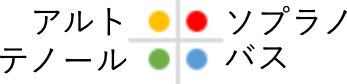
\includegraphics[scale=.7]{images/subjectiveExp/scat_0_legend.jpg}
  \end{minipage}

  \begin{minipage}{0.5\linewidth}
    \centering
    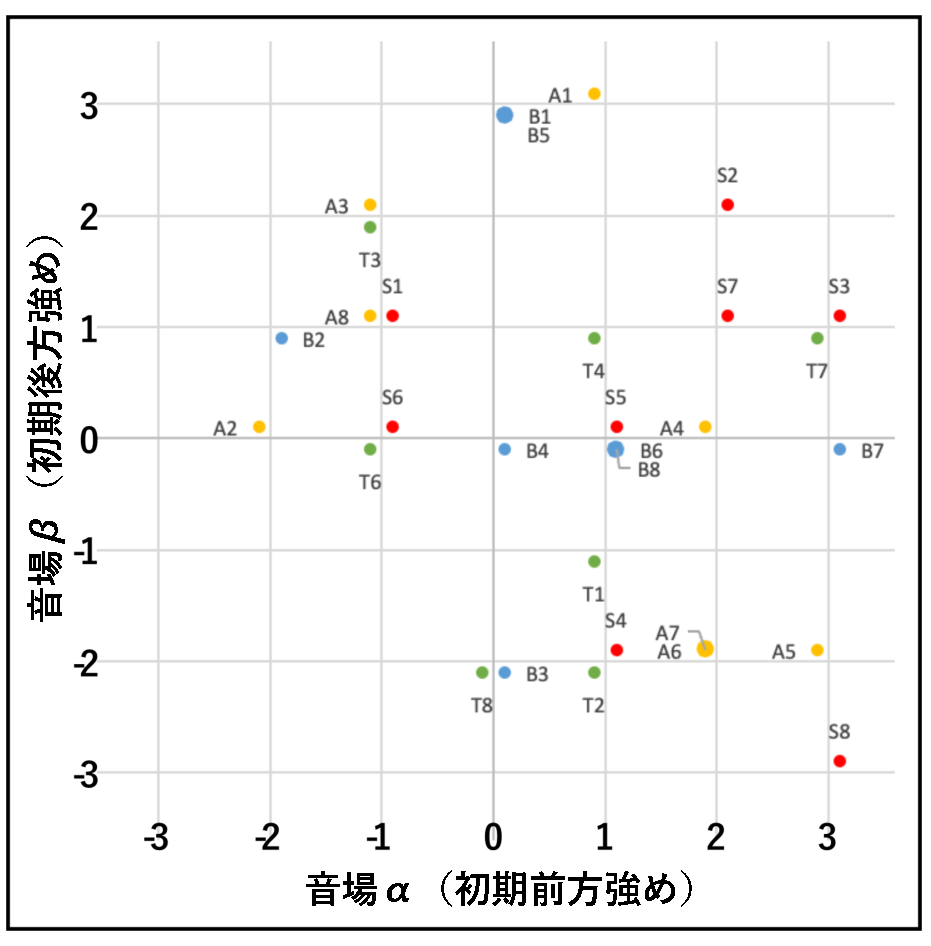
\includegraphics[width=.9\linewidth]{images/subjectiveExp/scat_early_01reverb.pdf}
    \caption*{響きが増えたか}
  \end{minipage}%
  \begin{minipage}{0.5\linewidth}
    \centering
    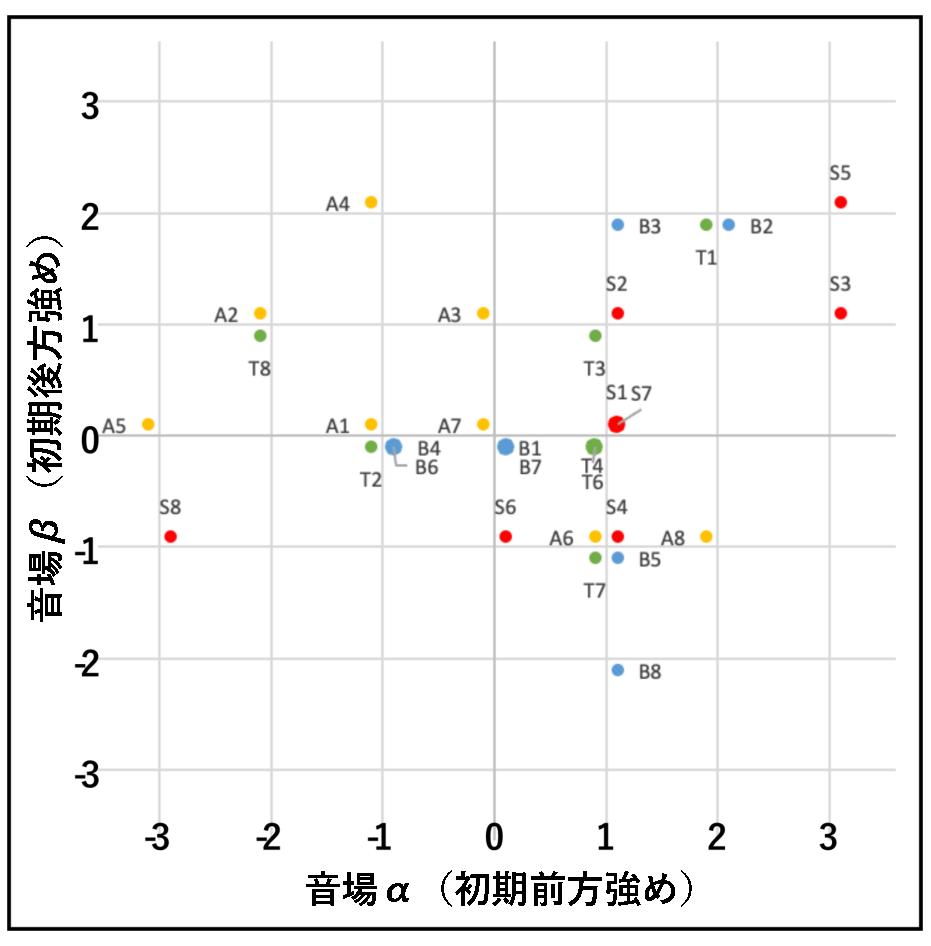
\includegraphics[width=.9\linewidth]{images/subjectiveExp/scat_early_02selfVoice.pdf}
    \caption*{自分の声の聴きやすさ}
  \end{minipage}

  \begin{minipage}{1\linewidth}
    \centering
    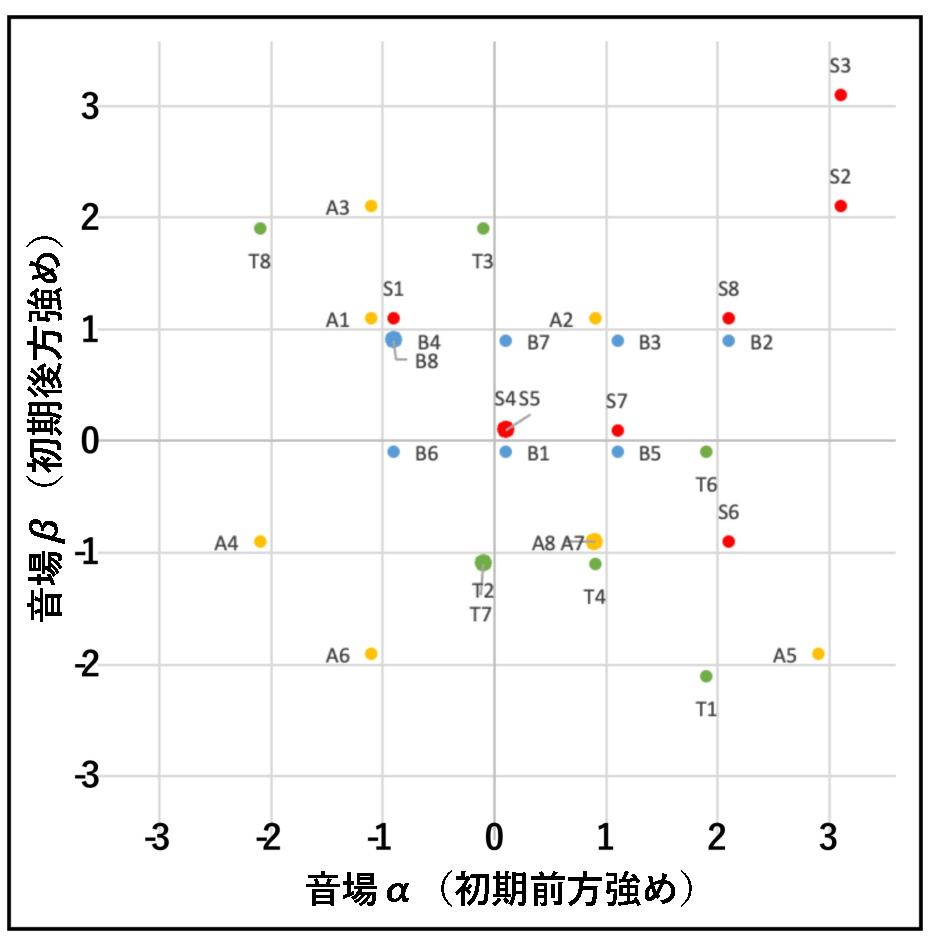
\includegraphics[width=.45\linewidth]{images/subjectiveExp/scat_early_03othersVoice.pdf}
    \caption*{他人の声の聴きやすさ}
  \end{minipage}
  \caption{響きの印象に関する評価の散布図}
  \label{fig:響きの印象に関する評価の散布図}
\end{figure}

%=======================================================================
\newpage
\subsubsection*{初期反射音の方向特性による空間の印象の変化}
いずれの評価項目でも、被験者の評価は広く分布しており、初期反射音の方向特性は空間の印象に対して個人差を生じさせる要因であると考えられる。また、「空間の広がり」については音場αに対するソプラノの評価が高い傾向にあった。初期反射音の供給のためにソプラノ側のスピーカーからの音が増幅されている可能性があり、そうであれば、そのことが空間の広がりに対して有意な影響を与えている可能性が大いに考えられる。

\vspace{\stretch{1}}

\begin{figure}[H]
  \begin{minipage}{1\linewidth}
    \centering
    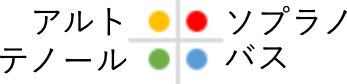
\includegraphics[scale=.7]{images/subjectiveExp/scat_0_legend.jpg}
  \end{minipage}

  \begin{minipage}{0.5\linewidth}
    \centering
    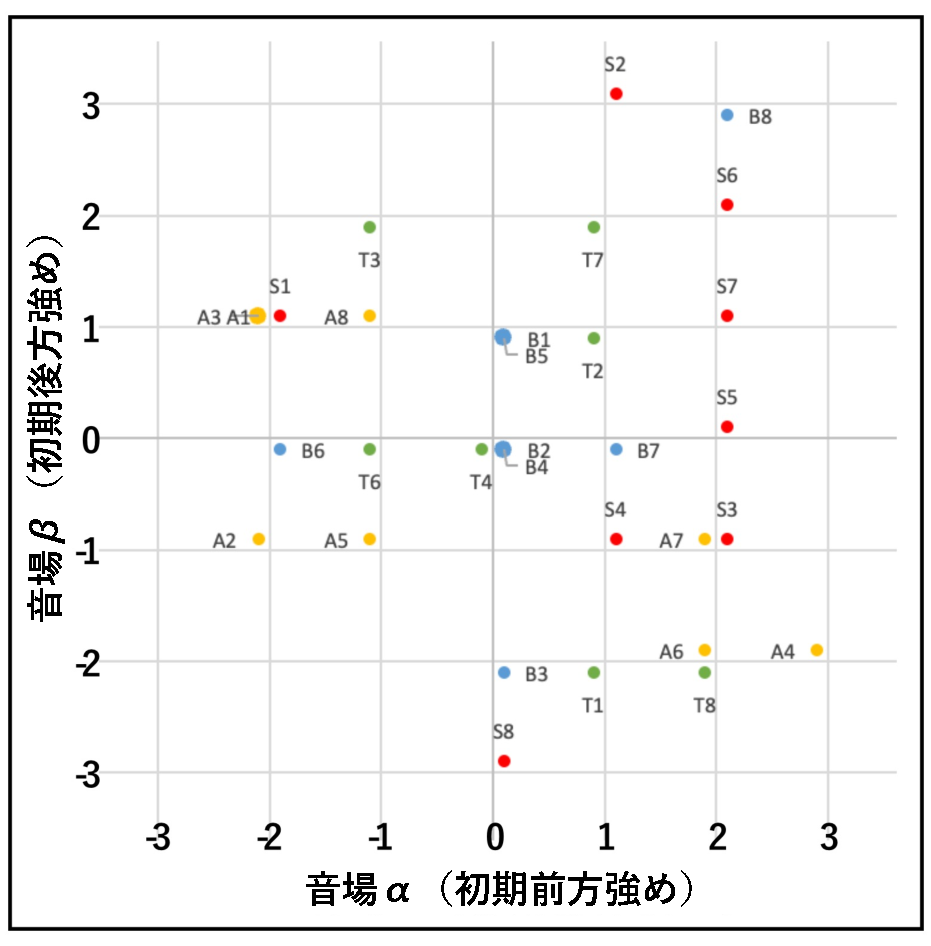
\includegraphics[width=.9\linewidth]{images/subjectiveExp/scat_early_04spacy.pdf}
    \caption*{空間の広がり}
  \end{minipage}%
  \begin{minipage}{0.5\linewidth}
    \centering
    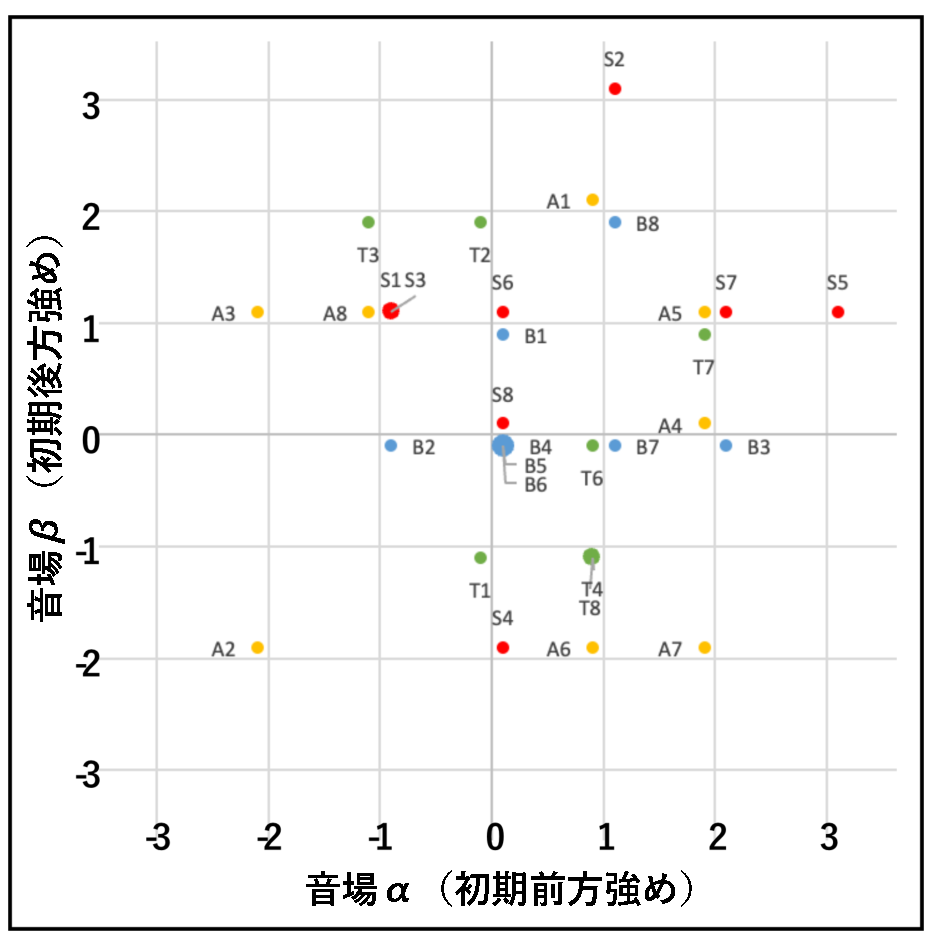
\includegraphics[width=.9\linewidth]{images/subjectiveExp/scat_early_05audience.pdf}
    \caption*{客席全体に届いている感じ}
  \end{minipage}
  \begin{minipage}{.5\linewidth}
    \centering
    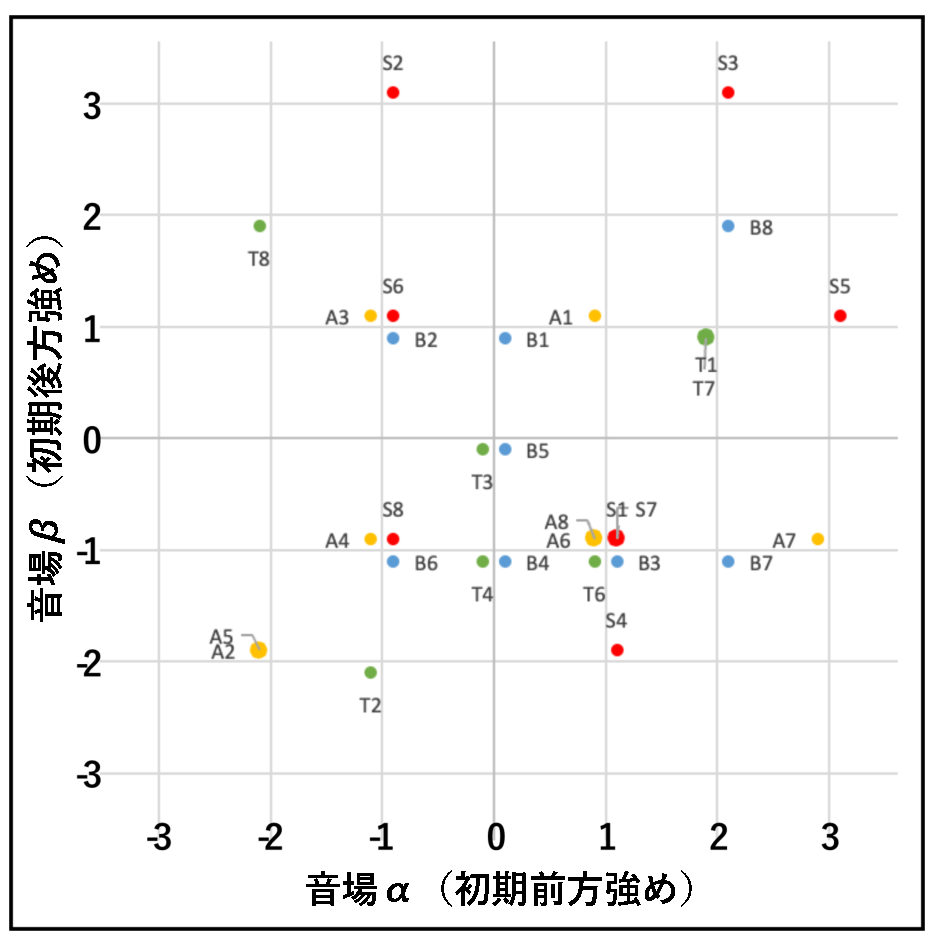
\includegraphics[width=.9\linewidth]{images/subjectiveExp/scat_early_06returnSelf.pdf}
    \caption*{自分に音が返る感じ}
  \end{minipage}%
  \begin{minipage}{.5\linewidth}
    \centering
    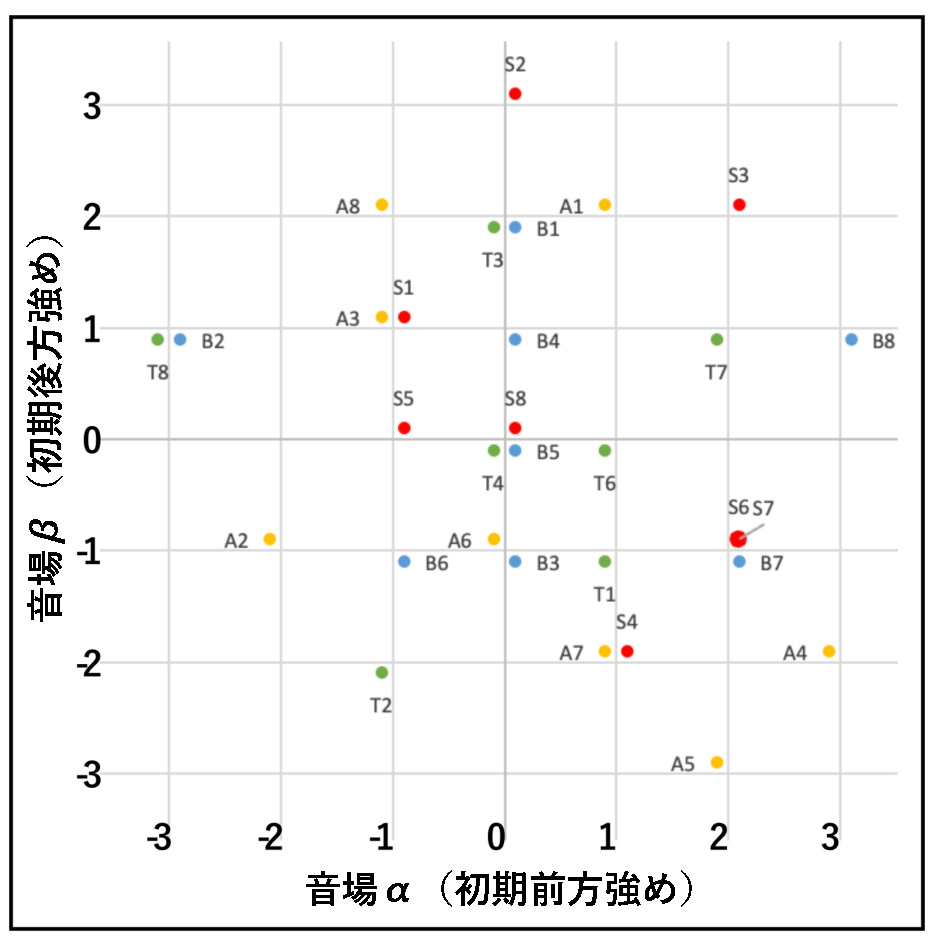
\includegraphics[width=.9\linewidth]{images/subjectiveExp/scat_early_07surrounded.pdf}
    \caption*{音に包まれる感じ}
  \end{minipage}

  \caption{空間の印象に関する評価の散布図}
  \label{fig:空間の印象に関する評価の散布図}
\end{figure}

\vspace{\stretch{1}}

%=======================================================================
\newpage
\subsubsection*{初期反射音の方向特性による演奏の印象の変化}
空間の印象に関する評価項目では被験者が広く分布していたのに対し、演奏の印象に関する評価項目では被験者の評価は中央付近に集中している傾向が見られた。演奏の印象に対する初期反射音の方向特性による影響は多くの演奏者にとって共通して小さい傾向にあると考えられる。「疲れ感」については被験者のばらつきが特に小さく、初期反射音の方向特性による影響はほとんどないと考えられる。

\vspace{\stretch{1}}

\begin{figure}[H]
  \begin{minipage}{1\linewidth}
    \centering
    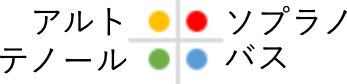
\includegraphics[scale=.7]{images/subjectiveExp/scat_0_legend.jpg}
  \end{minipage}

  \begin{minipage}{0.5\linewidth}
    \centering
    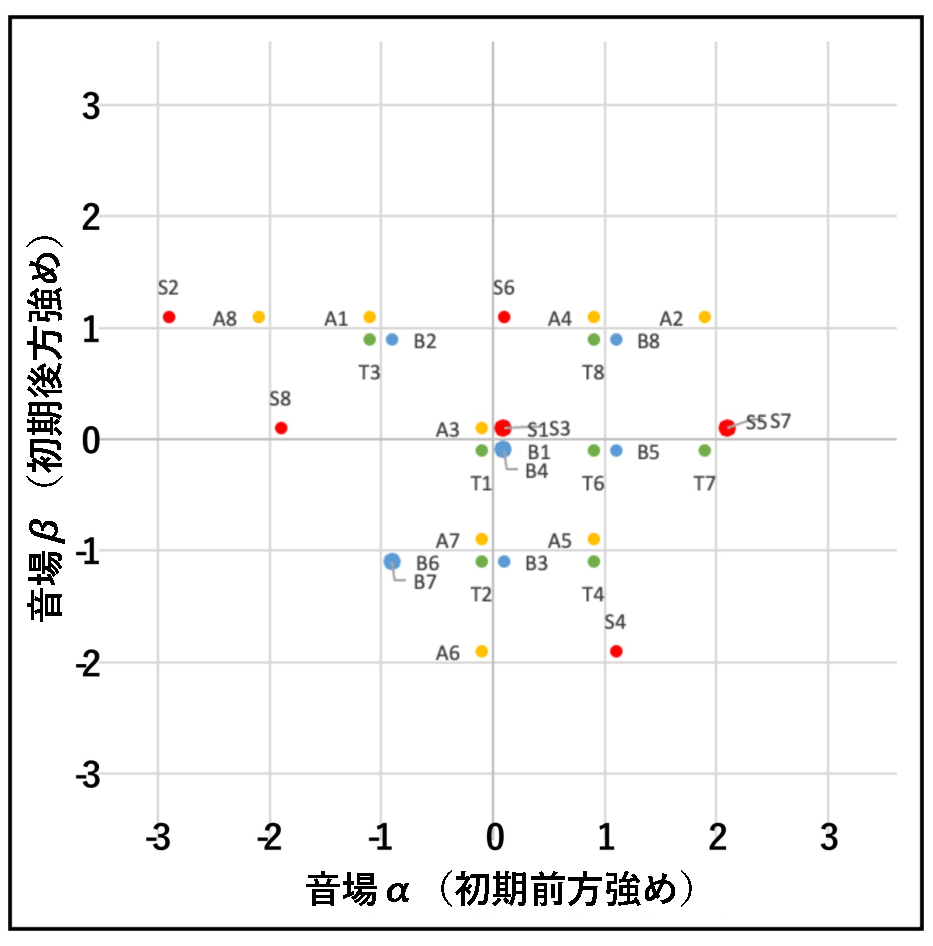
\includegraphics[width=.9\linewidth]{images/subjectiveExp/scat_early_08tiredness.pdf}
    \caption*{疲れ感}
  \end{minipage}%
  \begin{minipage}{0.5\linewidth}
    \centering
    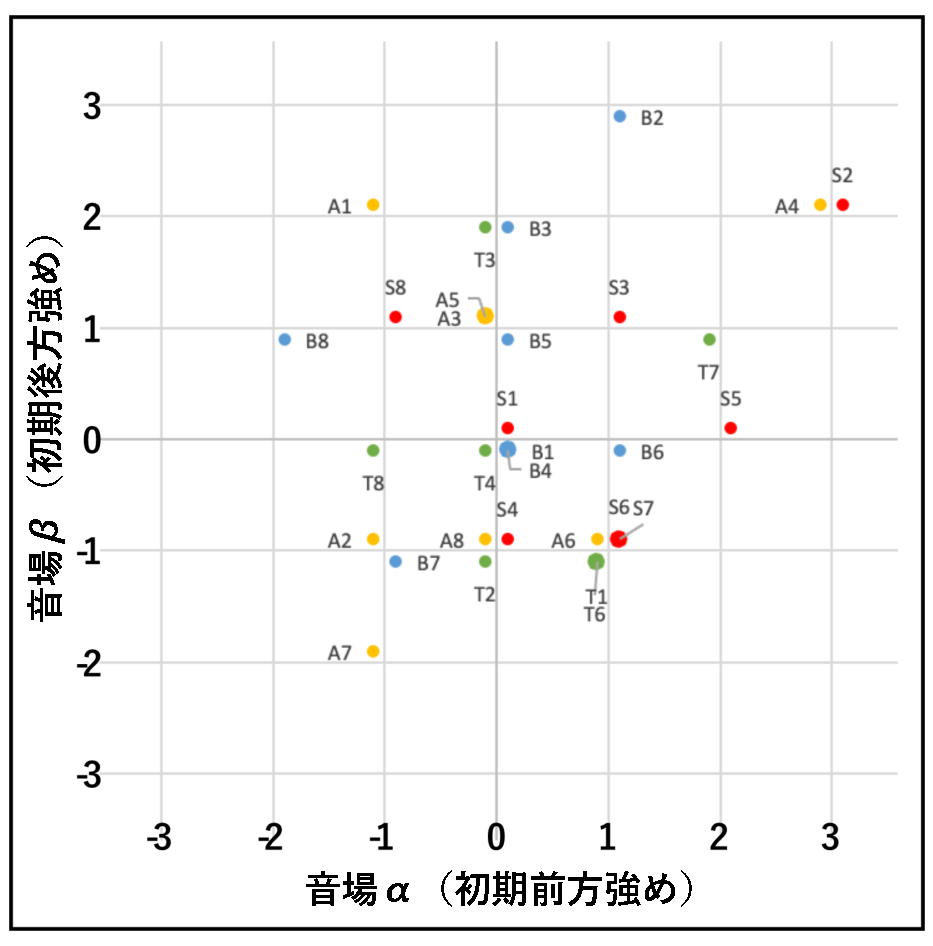
\includegraphics[width=.9\linewidth]{images/subjectiveExp/scat_early_09dynamics.pdf}
    \caption*{強弱の付けやすさ}
  \end{minipage}
  \begin{minipage}{.5\linewidth}
    \centering
    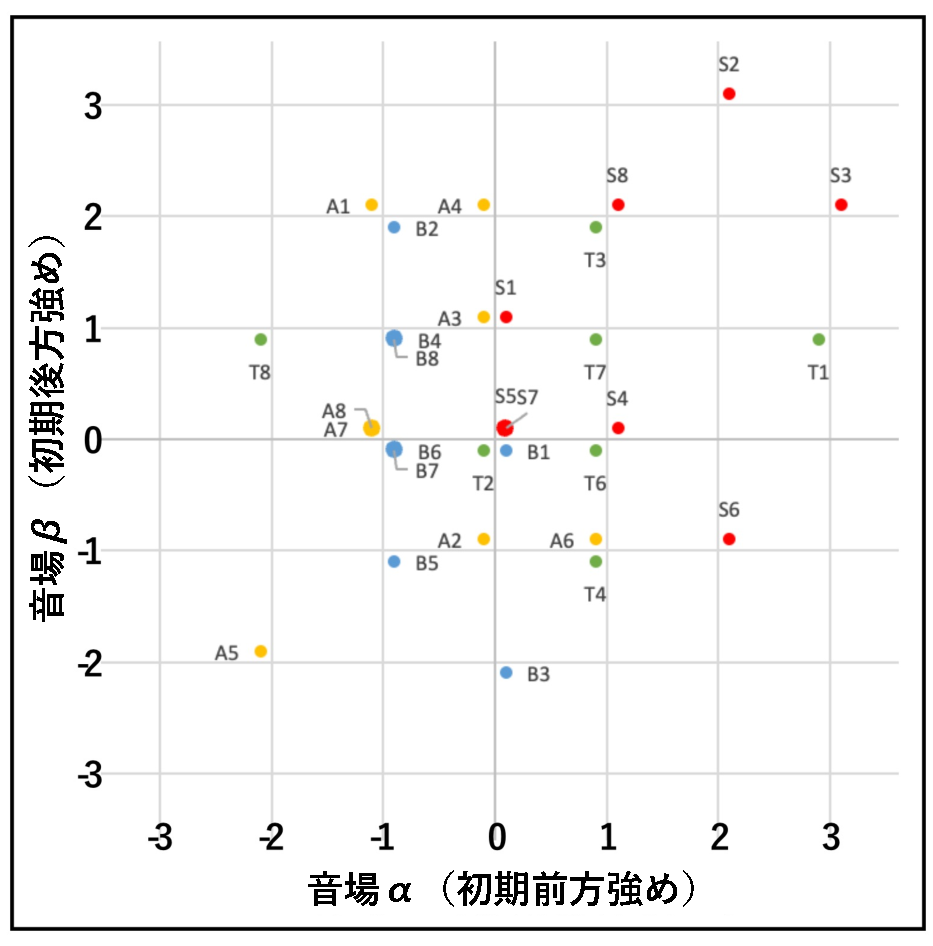
\includegraphics[width=.9\linewidth]{images/subjectiveExp/scat_early_10ensemble.pdf}
    \caption*{アンサンブルのしやすさ}
  \end{minipage}%
  \begin{minipage}{.5\linewidth}
    \centering
    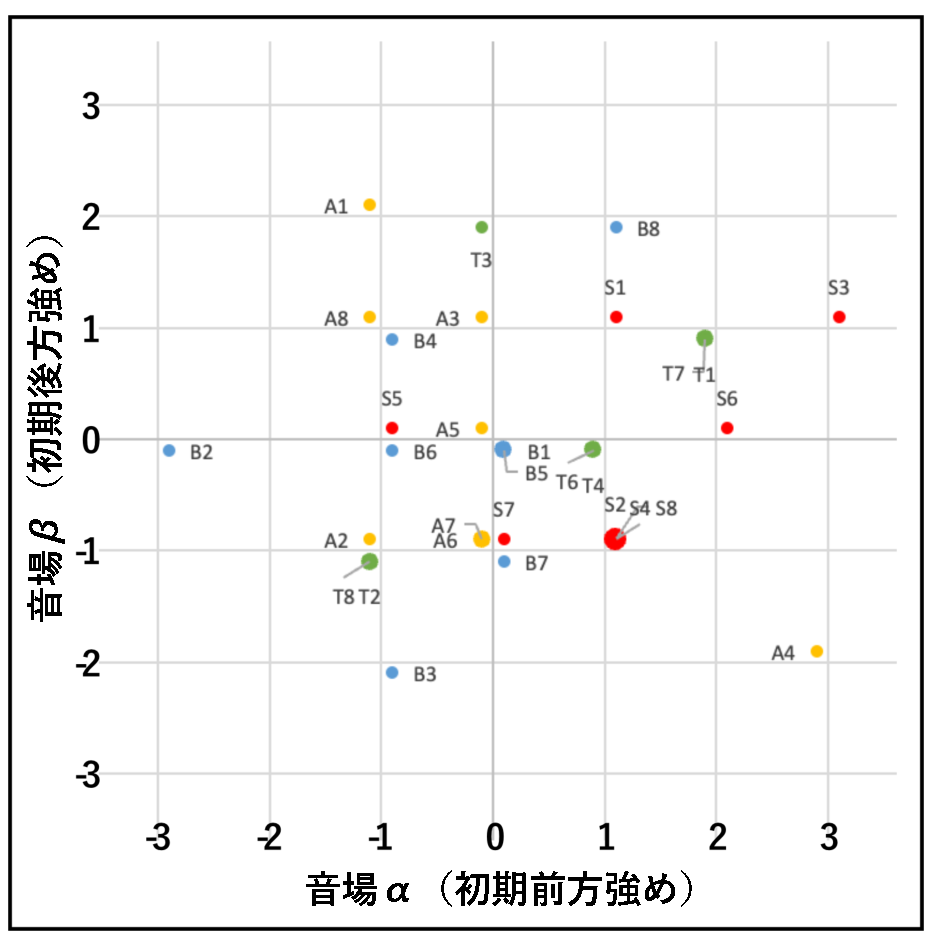
\includegraphics[width=.9\linewidth]{images/subjectiveExp/scat_early_11notConflict.pdf}
    \caption*{溶け合い感}
  \end{minipage}

  \caption{演奏の印象に関する評価の散布図}
  \label{fig:演奏の印象に関する評価の散布図}
\end{figure}

\vspace{\stretch{1}}
%=======================================================================
\newpage
\subsubsection*{初期反射音の方向特性による総合的な評価の変化}
「演奏がうまくいったか」「演奏のしやすさ」のどちらの項目でも、音場βの評価は0付近に集中しているのに対し、音場αの評価は広く分布していた。音場αの評価において、ソプラノの評価が高くアルトの評価が低い傾向はある程度はっきりと見られた一方で、テノールとバスのばらつきの傾向はあまり顕著でなかった。

\vspace{\stretch{1}}

\begin{figure}[H]
  \begin{minipage}{1\linewidth}
    \centering
    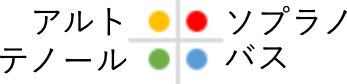
\includegraphics[scale=.7]{images/subjectiveExp/scat_0_legend.jpg}
  \end{minipage}

  \begin{minipage}{0.5\linewidth}
    \centering
    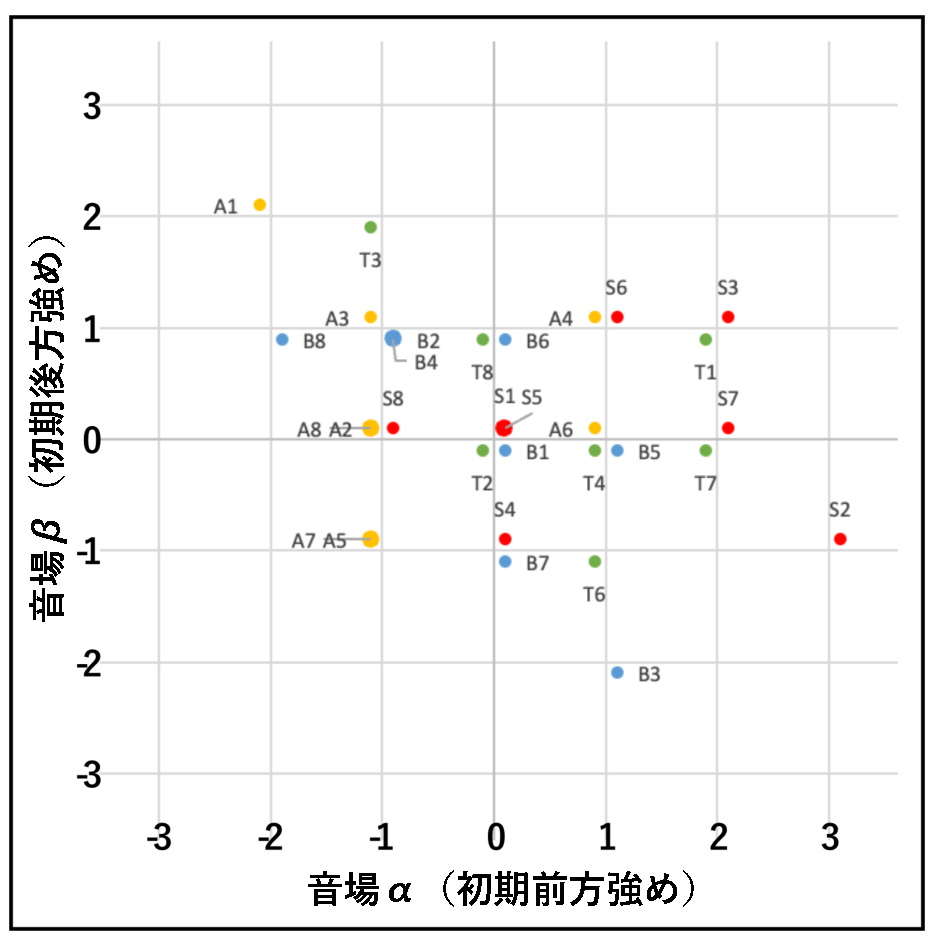
\includegraphics[width=.9\linewidth]{images/subjectiveExp/scat_early_12wellDone.pdf}
    \caption*{演奏がうまくいったか}
  \end{minipage}%
  \begin{minipage}{0.5\linewidth}
    \centering
    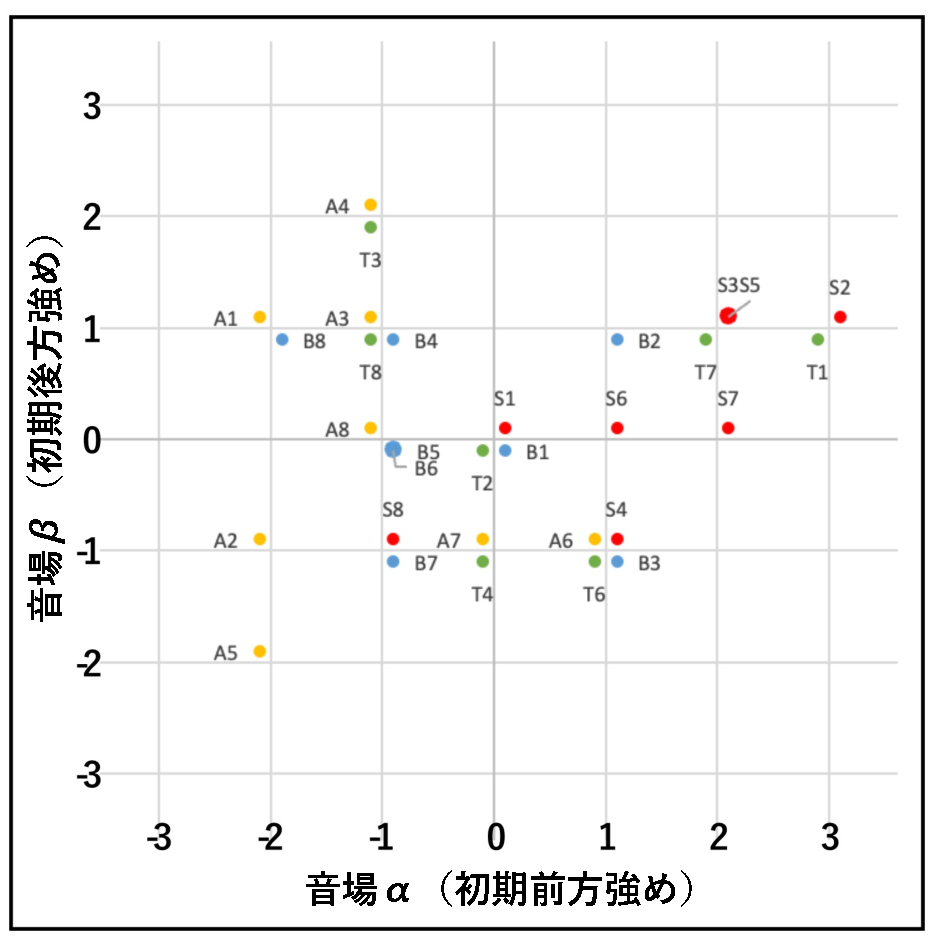
\includegraphics[width=.9\linewidth]{images/subjectiveExp/scat_early_13easiness.pdf}
    \caption*{演奏のしやすさ}
  \end{minipage}

  \caption{総合的な評価の散布図}
  \label{fig:総合的な評価の散布図}
\end{figure}

\vspace{\stretch{1}}
%=======================================================================
\newpage

\subsubsection*{後期反射音の方向特性による響きの印象の変化}
「響きが増えたか」の評価項目では、音場δの評価が全体的に高くなった。また、「他人の声の聴きやすさ」では、音場γ、音場δともに評価が全体的に高くなっている。$ST_{Late}$と残響時間は音場α、β、γ、δで大きく異なっていないため、これらの評価の向上は後期反射音の方向特性によるものと考えられ、後方からの後期反射音供給の増加が響き感や他人の声の聴きやすさを向上させ、また前方からの後期反射音供給の増加も他人の声の聴きやすさを向上させることが示唆される。

\vspace{\stretch{1}}

\begin{figure}[H]
  \begin{minipage}{1\linewidth}
    \centering
    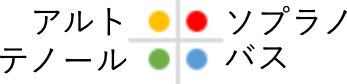
\includegraphics[scale=.7]{images/subjectiveExp/scat_0_legend.jpg}
  \end{minipage}

  \begin{minipage}{0.5\linewidth}
    \centering
    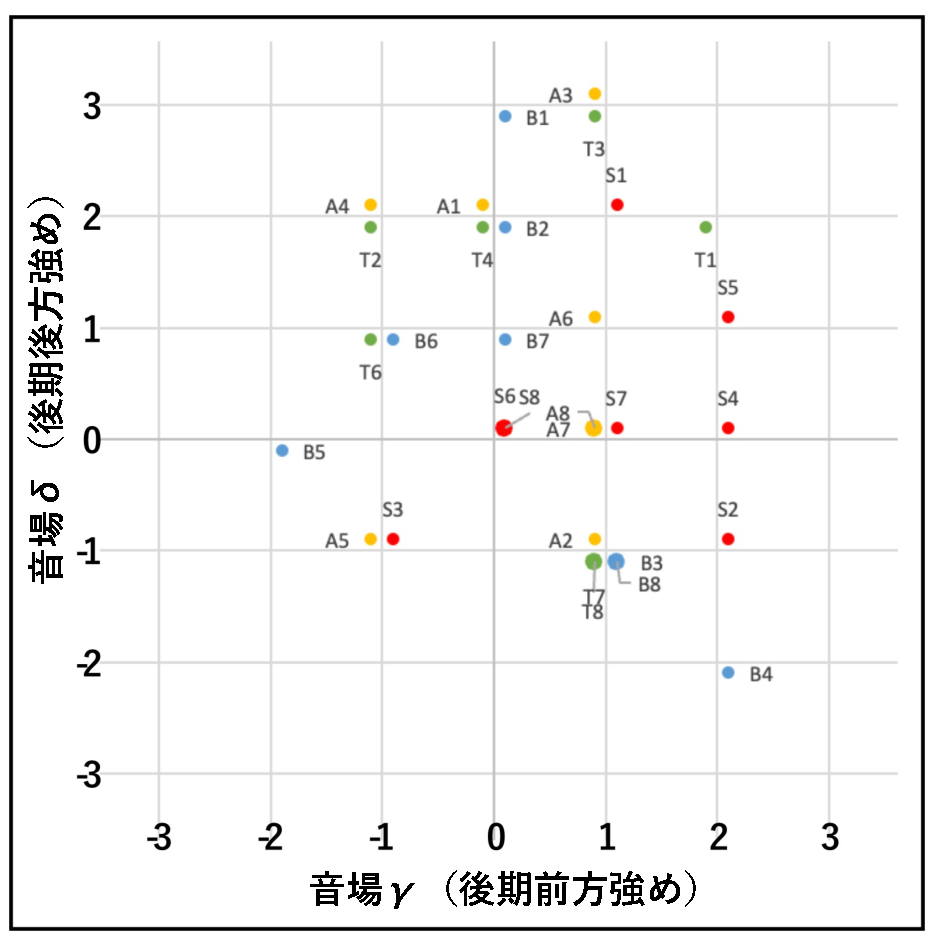
\includegraphics[width=.9\linewidth]{images/subjectiveExp/scat_late_01reverb.pdf}
    \caption*{響きが増えたか}
  \end{minipage}%
  \begin{minipage}{0.5\linewidth}
    \centering
    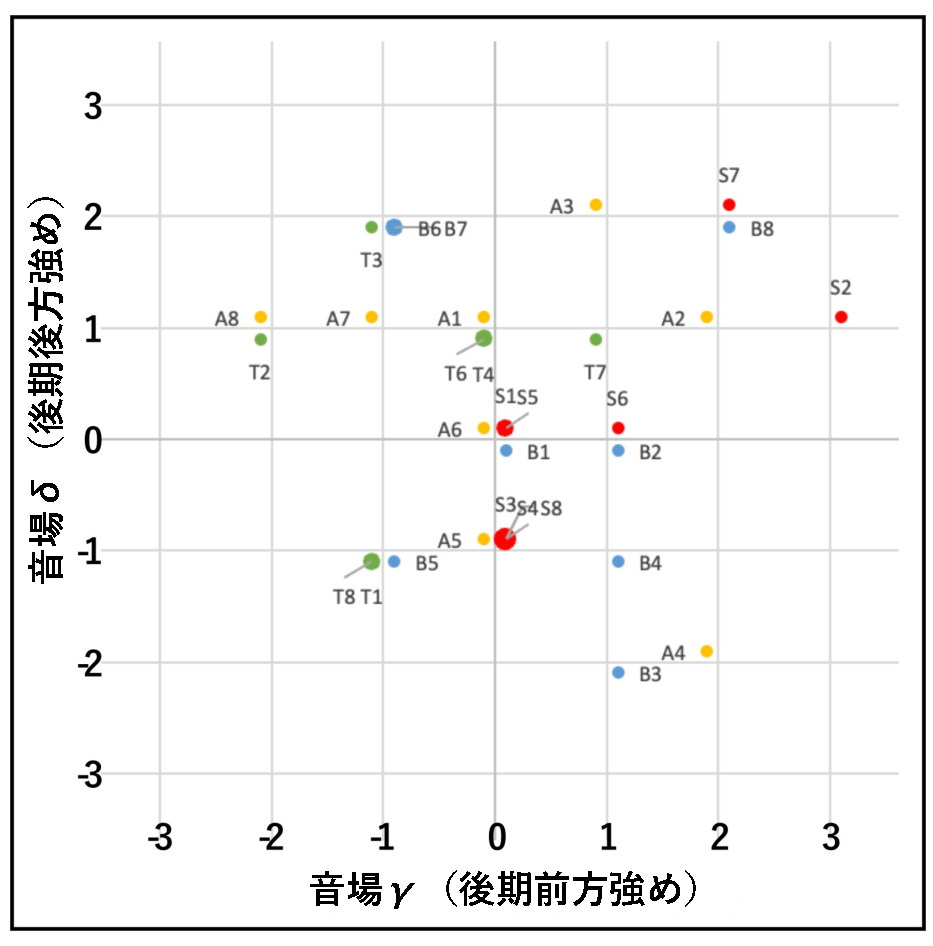
\includegraphics[width=.9\linewidth]{images/subjectiveExp/scat_late_02selfVoice.pdf}
    \caption*{自分の声の聴きやすさ}
  \end{minipage}

  \begin{minipage}{1\linewidth}
    \centering
    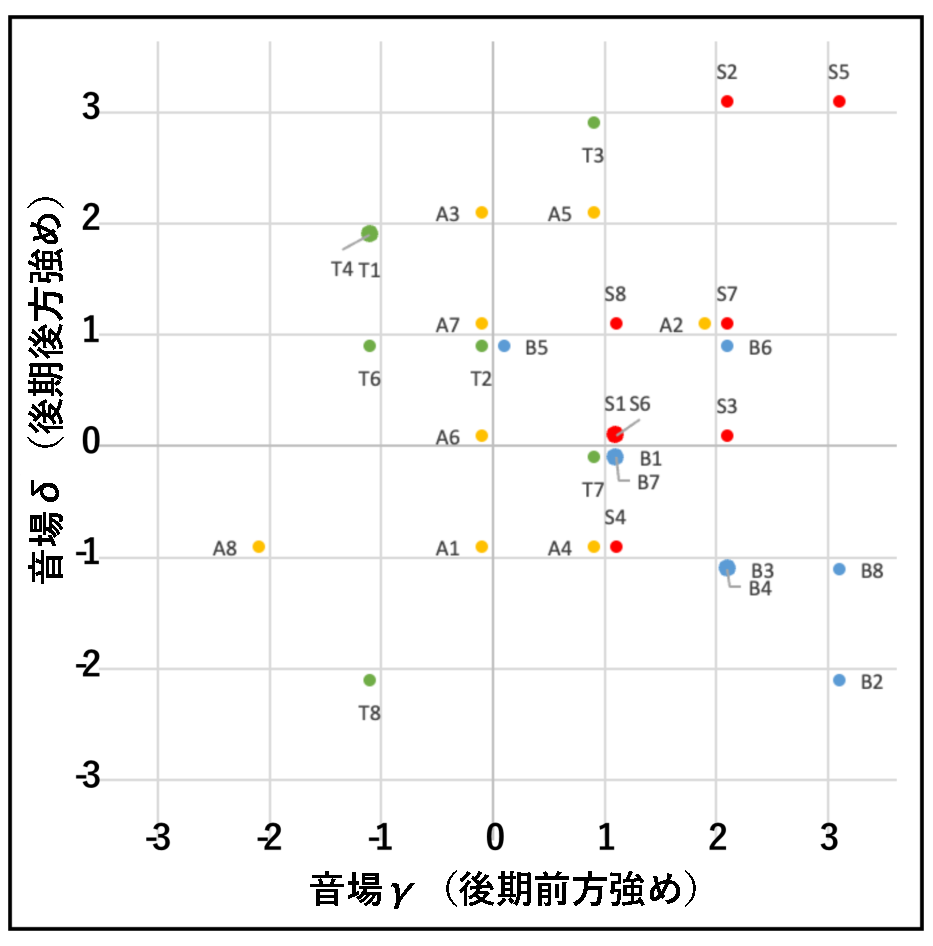
\includegraphics[width=.45\linewidth]{images/subjectiveExp/scat_late_03othersVoice.pdf}
    \caption*{他人の声の聴きやすさ}
  \end{minipage}
  \caption{響きの印象に関する評価の散布図}
  \label{fig:響きの印象に関する評価の散布図}
\end{figure}

\vspace{\stretch{1}}

%=======================================================================
\newpage
\subsubsection*{後期反射音の方向特性による空間の印象の変化}
「自分に音が返る感じ」「音に包まれる感じ」の2項目では、散布図に負の相関が見られた。音場γを高く評価した被験者の自由記述を見ると、「客席で聞こえる音をモニターしているよう」「残響が前に伝わる感触があった」などの客席での聴こえ方や客席への届き方を意識した記述が見られた。一方、音場δを高く評価した被験者では、「響きの残り具合がホールっぽい」「周囲からの反響をよく聴けた」「他パートの声がよく聴こえた」といったステージ上の自分の周囲の音に対する意識からくる記述が見られた。これらの記述から、ここでの評価傾向の差異は被験者ごとの意識の置き方の差異に起因している可能性が示唆される。

\vspace{\stretch{1}}

\begin{figure}[H]
  \begin{minipage}{1\linewidth}
    \centering
    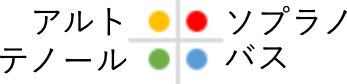
\includegraphics[scale=.7]{images/subjectiveExp/scat_0_legend.jpg}
  \end{minipage}

  \begin{minipage}{0.5\linewidth}
    \centering
    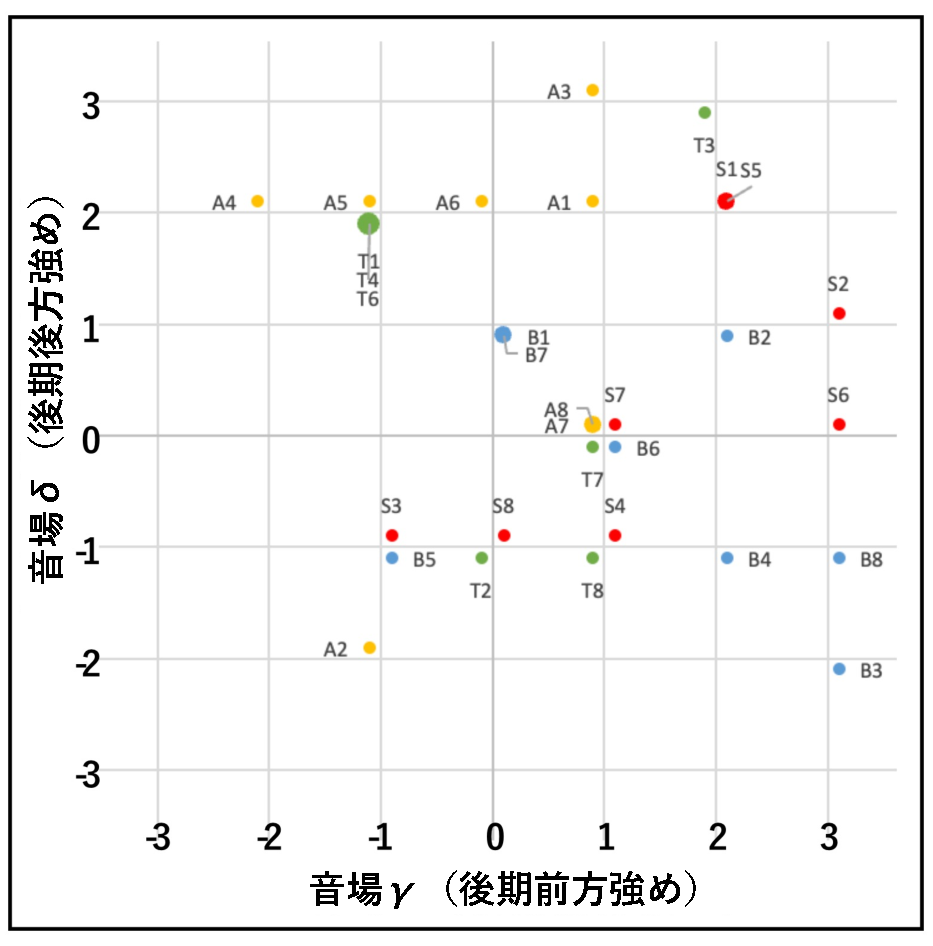
\includegraphics[width=.9\linewidth]{images/subjectiveExp/scat_late_04spacy.pdf}
    \caption*{空間の広がり}
  \end{minipage}%
  \begin{minipage}{0.5\linewidth}
    \centering
    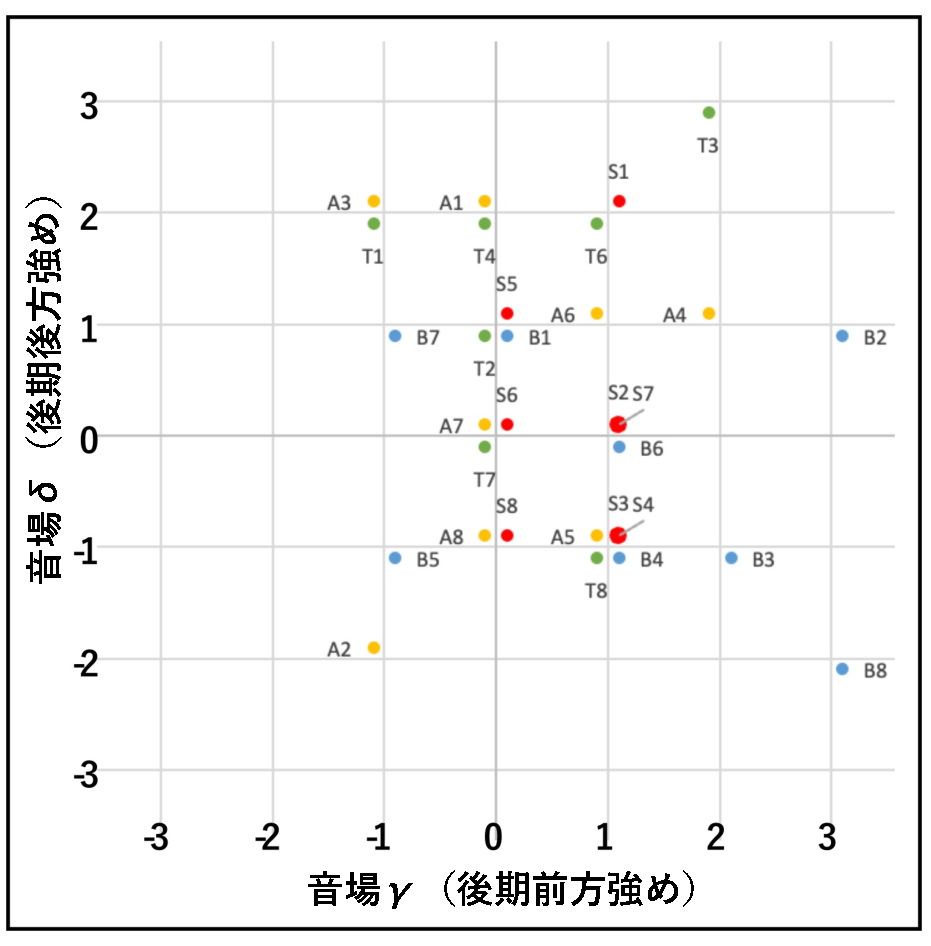
\includegraphics[width=.9\linewidth]{images/subjectiveExp/scat_late_05audience.pdf}
    \caption*{客席全体に届いている感じ}
  \end{minipage}
  \begin{minipage}{.5\linewidth}
    \centering
    \includegraphics[width=.9\linewidth]{images/subjectiveExp/scat_late_06returnSelf.pdf}
    \caption*{自分に音が返る感じ}
  \end{minipage}%
  \begin{minipage}{.5\linewidth}
    \centering
    \includegraphics[width=.9\linewidth]{images/subjectiveExp/scat_late_07surrounded.pdf}
    \caption*{音に包まれる感じ}
  \end{minipage}

  \caption{空間の印象に関する評価の散布図}
  \label{fig:空間の印象に関する評価の散布図}
\end{figure}

\vspace{\stretch{1}}

%=======================================================================
\newpage
\subsubsection*{後期反射音の方向特性による演奏の印象の変化}
「疲れ感」については、音場γ、δともに評価が0付近に集中していた。この傾向は初期反射音の方向特性を変化させたときも同様であり、疲れ感に対する反射音の方向特性による影響はほとんどないと考えられる。「強弱の付けやすさ」「アンサンブルのしやすさ」2項目については、評価が散布図の右上に寄っている傾向が見られ、後期反射音の前方・後方いずれの供給量の増加も演奏の印象を向上させる可能性があることが示唆された。しかし、この2項目と「溶け合い感」を合わせた3項目では、音場γと音場δの両方を高く評価した人は多くなく、多くの被験者が音場γと音場δのいずれか一方を高く評価していた。

\vspace{\stretch{1}}

\begin{figure}[H]
  \begin{minipage}{1\linewidth}
    \centering
    \includegraphics[scale=.7]{images/subjectiveExp/scat_0_legend.jpg}
  \end{minipage}

  \begin{minipage}{0.5\linewidth}
    \centering
    \includegraphics[width=.9\linewidth]{images/subjectiveExp/scat_late_08tiredness.pdf}
    \caption*{疲れ感}
  \end{minipage}%
  \begin{minipage}{0.5\linewidth}
    \centering
    \includegraphics[width=.9\linewidth]{images/subjectiveExp/scat_late_09dynamics.pdf}
    \caption*{強弱の付けやすさ}
  \end{minipage}
  \begin{minipage}{.5\linewidth}
    \centering
    \includegraphics[width=.9\linewidth]{images/subjectiveExp/scat_late_10ensemble.pdf}
    \caption*{アンサンブルのしやすさ}
  \end{minipage}%
  \begin{minipage}{.5\linewidth}
    \centering
    \includegraphics[width=.9\linewidth]{images/subjectiveExp/scat_late_11notConflict.pdf}
    \caption*{溶け合い感}
  \end{minipage}

  \caption{演奏の印象に関する評価の散布図}
  \label{fig:演奏の印象に関する評価の散布図}
\end{figure}

\vspace{\stretch{1}}

%=======================================================================
\newpage
\subsubsection*{後期反射音の方向特性による総合的な評価の変化}

「演奏がうまくいったか」の項目については、音場γ、δともに変化を少ないとした回答が多く、演奏者自身が環境に応じて演奏することに慣れていることが窺える。一方で「演奏のしやすさ」には音場γ、δともに評価にはばらつきが大きかった。特に音場γでは評価の平均値が高いこと から、後期残響音の前方からの供給量が大きい音場が好まれることが示唆された。

\vspace{\stretch{1}}

\begin{figure}[H]
  \begin{minipage}{1\linewidth}
    \centering
    \includegraphics[scale=.7]{images/subjectiveExp/scat_0_legend.jpg}
  \end{minipage}

  \begin{minipage}{0.5\linewidth}
    \centering
    \includegraphics[width=.9\linewidth]{images/subjectiveExp/scat_late_12wellDone.pdf}
    \caption*{演奏がうまくいったか}
  \end{minipage}%
  \begin{minipage}{0.5\linewidth}
    \centering
    \includegraphics[width=.9\linewidth]{images/subjectiveExp/scat_late_13easiness.pdf}
    \caption*{演奏のしやすさ}
  \end{minipage}

  \caption{総合的な評価の散布図}
  \label{fig:総合的な評価の散布図}
\end{figure}

\vspace{\stretch{2}}

%=======================================================================

\clearpage

% 参考文献
% 参考文献の箇所にインプットしてください。

% 分割ファイル内でのみ,bibliographyを読み込みます。

\expandafter\ifx\csname ifdraft\endcsname\relax

  % bibliographyを展開する

  \bibliographystyle{junsrt}
  \bibliography{ref.bib}% 同じディレクトリ内のbibファイルのみを参照可能

\fi

\end{document}